%
%                       This is a LaTeX 2e version of the
%                       laboratory project template file.
%\documentclass{aa}
\documentclass[a4paper,12pt]{article}
%\usepackage{fullpage,epsf}
%
%                       This subsection generates a title page
%                       Edit only the subsections indicated to put
%                       in the project title, your name, supervisor,
%                       project length in weeks and submission date
\usepackage[english]{babel}
\usepackage[utf8]{inputenc}
\usepackage{csquotes}% Recommended
\usepackage{amsmath,amssymb,latexsym}
\usepackage{graphicx}
\usepackage{subfig}
\usepackage{geometry}
\usepackage{lipsum}
\usepackage{epigraph}
\usepackage[table,xcdraw]{xcolor}
\usepackage{multirow}

\setlength{\parindent}{2em}
\setlength{\parskip}{1em}
%\usepackage{biblatex}
\usepackage{natbib}
\usepackage{aas_macros}
%\bibliographystyle{agsm}
\usepackage[nottoc,notlof,notlot]{tocbibind} 
\renewcommand\bibname{References}
\bibpunct{(}{)}{;}{a}{}{,} % to follow the 
\usepackage{listings}
\usepackage{color}

\definecolor{dkgreen}{rgb}{0,0.6,0}
\definecolor{gray}{rgb}{0.5,0.5,0.5}
\definecolor{mauve}{rgb}{0.58,0,0.82}

\lstset{
  language=Python,
  aboveskip=3mm,
  belowskip=3mm,
  showstringspaces=false,
  columns=flexible,
  basicstyle={\small\ttfamily},
  numbers=left,
  numberstyle=\tiny\color{gray},
  keywordstyle=\color{blue},
  commentstyle=\color{dkgreen},
  stringstyle=\color{mauve},
  breaklines=true,
  breakatwhitespace=true,
  tabsize=3,
  frame=single
}

\begin{document}
\pagestyle{empty}                       % No numbers of title page                      
%\epsfxsize=40mm                         % Size of crest
\begin{minipage}[b]{110mm}
        {\Huge\bf Computer and \\Information Sciences
        \vspace*{17mm}}
\end{minipage}
\hfill
\begin{minipage}[t]{40mm}               
        \makebox[40mm]{
        
\includegraphics[width=1\linewidth]{strath_logo.png}}
\end{minipage}
\par\noindent                                           % Centre Title, and name
\vspace*{0cm}
\begin{center}
        \Large\bf \Large\bf Dissertation\\
        \Large\bf MSc Software Development\\[10pt]                     % Change to MP/CP/Astro
        \LARGE\bf Automated Mutation Testing for Concurrent Software         % Change to suit
\end{center}
\vspace*{0cm}
\begin{center}
        \bf Patrick Gray\\                           % Replace with your name
        August 2019                                    % Submission Date
\end{center}
\vspace*{5mm}
%
%                       Insert your abstract HERE
%                       
\begin{abstract}

\end{abstract}
\vspace*{2cm}
Signature:\hspace*{8cm}Date: 19/08/2019

\vfill
{\bf Supervisor:} Kostas Liaskos             % Change to suit
\hfill
                                       % Change to suit
\newpage

%
%                       End of Title Page
\pagestyle{plain}                               % Page numbers at bottom
\setcounter{page}{1}                            % Set page number to 1
\tableofcontents                                % Makes Table of Contents

\newpage
\section{Introduction}

\newpage
\section{Background}

The relevant background information required for this project will be presented here, as well as a review of the literature covering concurrent bug patterns and mutation operators. An overview of concurrency in Java and mutation testing for general software will provide the necessary understanding for the motivation of this project.  


\subsection{Concurrency}
\subsubsection{Threads}

Processes are self contained execution environments with private resources; most Java applications only require a single process to run efficiently. Modern computer systems provide multiple cores to process parallel execution of processes. Concurrency utilises this functionality with the use of \textit{Threads}. Threads are light-weight processes that share their resources (memory, open files, etc) with the other threads contained within the process \citep{mois15}. With the advancement of technology producing evermore powerful machines, each individual core has the ability to interleave multiple threads as well as the capability of running threads in parallel on separate cores. 

Creating threads is lighter on resources than creating new processes and the ability to share resources is beneficial to performance. This is the main motivation for using concurrent code; allowing multiple sections of code to run simultaneously for faster execution times. Another positive aspect of this is the improved responsiveness of a system \citep{peierls05}. When one section of a program becomes blocked or slows down, a single threaded system would become unresponsive to the user and would report no information back to explain why. A multi-threaded application would allow a computationally greedy operation to perform in the background without disrupting the rest of the system and remaining responsive to observation and interaction from the user.

Each program has at least one thread, the main thread, created at point of calling the main() method, but subsequent threads can be created after this execution. There are two ways to create new instances of threads. The first is to create an object that has implemented the Runnable interface and pass this to the Thread constructor. The thread will then execute the run() method of the runnable object. The other is to create an object that is a subclass of Thread and executing the run() method pertaining to the object \citep{concurrency19}. In both cases, Thread.start() must be executed to start a specified instance of a thread. Although, threads are not necessarily run in the order of their start() execution, the threads are automatically assigned a priority by the Java Vitrual Machine (JVM), and scheduled in order of highest priority \citep{mois15}. The first instance is a more general and flexible approach since it is implementing the Runnable interface, it allows for the class to inherit functionality from another class. This also has the benefit of allowing its own parameters to be passed to the constructor. The second is easier to use in simple applications, but since it is a subclass of Thread, there are limitations to what the class can do, as only the parent class Thread constructors are available. 

If a thread wants another thread to stop then it can invoke an interruption using Thread.interrupt(), which will throw an exception message to the interrupted thread. A thread can support its own interruption by invoking the sleep() method to stop itself for a specified period of time. After the elapsed time, the thread will resume running, unless an interrupt is called and the thread is terminated. Sleep() can be used by the user to manage the scheduling of threads if it is prescient for a particular operation and limits the unpredictability of the system behaviour. Similar to a thread sleep, Thread.join() can be used for one Thread to wait until another has completed its execution. With no specified time, the Thread may wait indefinitely for the other one to terminate. 


\subsubsection{Atomic Operations} \label{section:atmoic}

An atomic operation is one that is executed and completed all at once or not at all \citep{concurrency19}. It is an action that is considered safe from interference from other operations, as it cannot be stopped during execution and the state of the process cannot be changed by another operation: the state is only affected by the atomic operation from the start to finish. A single line of code does not imply atomicity, no matter how deceptively simple it may appear. For instance, the increment operation for some integer, x++, is actually three separate operations handled by the Java Virtual Machine. First the value of the integer must be fetched, then it is incremented and finally the new value is written back to memory. This may seem trivial, but if mishandled, this can have unexpected and varying results if it is executed in conjunction with another Thread that is accessing the same data. When two threads interleave in such a way, it is referred to as interference. As an example, Thread A and Thread B are tasked to perform the increment operation on x. If they were to run consecutively, allowing for complete execution of the first operation before the initiating the next, the value of x would be expected to have increased by 2. However, if the two operations are executed at the same time, the following scenario could feasibly occur:
\begin{enumerate}
    \item Thread A retrieves the value of x, x = 0.
    \item Thread A increments x, x = 1.
    \item Thread B retrieves the value of x before the Thread A has been given the chance to commit the change of x to memory and thus, x remains equal to 0.
    \item Thread A stores the result of x = 1.
    \item Thread B increments x to 1 and stores the result. Despite two instances of incrementing the value of x, the final value is recorded as 1; the first instance has been overridden by the second.
\end{enumerate}

\begin{table}[]
    \centering
    \begin{tabular}{||l c||} 
     \hline
     Operation & Value of x  \\ 
     \hline\hline
     Thread A retrieves x & 0 \\ 
     \hline
     Thread A increments x & 1  \\
     \hline
     Thread B retrieves x & 0 \\
     \hline
     Thread A stores value of x & 1 \\
     \hline
     Thread B increments x & 1 \\  
     \hline
     Thread B stores value of x & 1 \\
     \hline
    \end{tabular}
    \caption{Example of a non-atomic operation, x++, in two interleaving threads.}
    \label{table:non-atomic}
\end{table}

 

This is only one small example of interference, but similar occurrences of inconsistent memory issues between threads can crop up throughout concurrent systems unless properly managed. Compounding this is the complexity of other scenarios with a greater number of interleaving threads and manipulation of more data. One method of preventing this is utilising the functionality of synchronized code, which will be explored in the following section.


\subsubsection{Synchronization and Locks}
    
Synchronization allows for critical sections of code or methods to be executed atomically with reference to code in other threads. The power of scheduling operations and resource management is passed to the user \citep{silberschatz13}. The synchronized keyword blocks other threads from executing simultaneously during its execution to ensure that the state of the system is only affected by the actions within the synchronized block. Synchronization can be applied to a specific set of actions in a block, specifying the resource to be restricted or to an entire method. The two methods of using the synchronized keyword are shown in Figure \ref{fig:synchronized}. 

\begin{figure}[h]
    \centering
    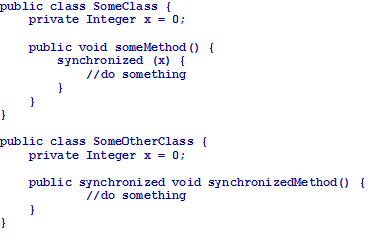
\includegraphics[scale = 0.8]{synchronized.png}
    \caption{Synchronized block and synchronized method}
    \label{fig:synchronized}
\end{figure}

Restricting the whole method will have a more dramatic effect on the performance as no other threads can run concurrently. Applying synchronization to the increment example would solve the observed problem of memory consistency and would guarantee the expected result to occur.

The synchronized keyword achieves the desired affect by imposing a lock on the synchronized block of code that prevents access to the contained object’s fields. After the synchronized block has terminated, the lock is released and normal thread scheduling will resume. Reentrant locks can be used to similar effect to the synchronized keyword, allowing a thread to obtain and release a lock during execution of critical code, much like a synchronized block of code. 

\subsubsection{Liveness}
The liveness of an application expresses its ability to execute without complications in an efficient manner. There are some issues that can interfere with the liveness of an application by slowing it down or even freeze functionality altogether. A deadlock can occur when two threads have locked separate resource, but are waiting on the other thread to release their lock to continue execution. 

\vspace{2pt}
\begin{center}
\noindent Thread 1: locks resource A, waits for resource B
\\Thread 2: locks resource B, waits for resource A 
\end{center}
\vspace{2pt}

In this instance, both resources are locked and unavailable for access until the other is released; the program will perpetually hang in an inescapable catch-22.  


\subsubsection{Executor Service}
Previously, concurrency examples provided have only involved two threads that are relatively simple to follow. In many cases, a program may wish to utilise many more threads for a significant boost in performance. The Java concurrent package offers the Executor Service to help maintain many instances of threads, a thread pool, by abstracting the management and construction of threads from the main program. This can be an invaluable tool for ensuring computation resources are not wasted by the constant creation of new threads for each concurrent action. Instead, a pool of threads is created at once and the threads will wait until they are required. After performing the necessary action, the thread will go back into a state of waiting for a request for work. The size of the pool has a specified limit, to prevent a runaway of thread creation; when all the threads in a pool are currently in use, the executor server will wait to assign work to the next available thread. Creating a thread takes up time and resources, it is far more efficient to recycle previously used threads. 


\subsection{Mutation Testing} \label{section:Mutation Testing}
Mutation testing is the process of seeding errors throughout a system’s codebase, to observe the effecting behaviour and evaluate the effectiveness of the present testing coverage \citep{adrion81}. A \textit{mutation operator} is a generalised rule, which describes the changes that will be made to a specific segment of code. The result of applying an operator to a code segment is known as a \textit{mutant} \citep{ammann17}. The premise of mutation testing is simple: if the previously implemented software tests have been designed adequately, then they should recognise the changes to the system behaviour and certain tests should fail accordingly. The mutation is referred to as killed in this instance. This is the ideal outcome when a mutation is applied to a system, as it suggests that the tests have been designed effectively and the coverage is sufficient. However, if a mutation survives by circumventing the tests, this indicates that the tests are either flawed or the test coverage has gaps and not all of the behaviour has been accounted for. This is a useful tool for highlighting weaknesses in test coverage; a full suite of unit tests that successfully pass when run on a system only informs the user that those specific function behaviours are expected. Although it provides no information on the behaviours that have been missed. Mutation testing aides identifying these areas of code that have been overlooked by applying many different mutations throughout the whole system, which should disrupt as much expected behaviour as possible. Thus, when a mutation is not successfully killed by any unit test, the location of the altered code will indicate that there is improvement to be made in the test coverage related to the affected area.

One example of a renowned mutation testing tool is Pitest (PIT)\footnote{}, which combines traditional line coverage with mutation coverage, to offer a comprehensive and fast testing environment for Java applications. The list of mutation operators it provides is extensive, covering relational operators (e.g. \textless, \textless=, \textgreater, \textgreater=), mathematical operators (e.g. +, -, *, etc.), logic statements a variety of different common method calls and return values \citep{pit19}. A mutation usually consists of altering a small section of code or removing a section entirely. For example, a conditional boundary operator would make the following mutation  in Figure \ref{fig:mutation}. 

\begin{figure}[h]
    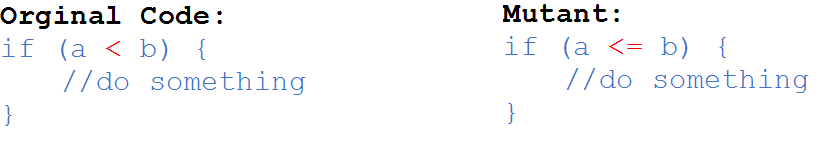
\includegraphics[scale = 0.65]{mutation.png}
    \caption{Relational operator mutation}
    \label{fig:mutation}
\end{figure}
    
The code now has a slightly different meaning. Designing effective unit tests involves specifically testing code at such boundary cases. The behaviour of the code would be monitored for values of a when less than b, equal to b and greater than b, with a separate test for each scenario. Prior to the mutation, the if statement would not be executed during runtime for when a is equal to b, but after the mutation the if statement would be entered. Thus, a unit test that previously would pass for this scenario should fail due to the alteration and the mutation could be considered successfully killed. PIT will apply many of these mutations on the byte code generated after compilation, instead of on the source files. This produces significantly faster runtimes. After mutation, PIT will automatically run the new java files against the designated unit tests and produce a set of results detailing the fates of each mutation. The varying states explained below:

\begin{description}
    \item[Killed - ]The mutation was successfully discovered by the presence of a failed unit test.
    \item[Lived -]The mutation was unsuccessfully discovered with no failed unit tests. 
    \item[No coverage -]The mutation lived because of a lack of unit tests covering the relevant mutated section of code. 
    \item[Non-viable -]The mutation affected the Java bytecode such that the JVM could not load the file.
    \item[Timed out -]The mutation created an infinite loop so execution of the file could not terminate. 
    \item[Memory error -]The mutation increased “the amount of memory used by the system or the result of the additional memory overhead required to repeatedly run your tests”.
    \item[Run error -]The mutation caused the file to be unable to run, similar to non-viable mutations.
\end{description}

The results detail which mutations were applied, identify which tests managed to kill mutations and produce the ratio of successfully caught mutations to the total number of seeded errors. This ratio is known as a \textit{mutation test score} \citep{bradbury06}. Although PIT offers a wide range of mutation operators, it is lacking in support for concurrent systems. Performing unit tests on multi-threaded code is not as straightforward as single-threaded.


\subsection{Regular Expressions}    

The theory of mutation testing has been presented, however the mechanism by which mutations are applied is not a simple process with a single approach. The method used in this project is a high-level approach, utilising regular expressions to identify and manipulate strings. This is a different approach to the method seen in the Pitest mutation tool; a more sophisticated and technically complex method operating on bytecode. For the size and scope of this project, performance is less of a concern, so manipulating source code is a viable option. 

Regular expressions, regex for short, are a syntactic description of a pattern, often used to search or manipulate strings in a text [cite]. Exact strings can be found with ease, but the true power behind regular expressions is the ability to search for generic patterns and manipulate any matches returned. The java.util.regex package allows a user defined pattern to be interpreted and will find any matches within a given text. This is primarily achieved using the Pattern and Matcher classes. Inputting a regular expression into a Pattern as a parameter will create a compiled version of the regex. The syntax of a pattern is built up of special character constructs that can match with independent characters or a defined range of characters. For example, a regex pattern could be used to search for a date in the following format DD month YYYY, i.e. 20 July 1969. This format has strict rules specifying that a date must consist of two digits followed by a word and finally four more digits. The regex can be made more complex by imposing more rules limiting the range of numbers for the day section to be between 1-31; the month section to only consist of the exact strings for the calendar months and the year section to be greater than 0000. All of this is achievable with the Java regex package. However, to keep it simple, the following regex example will only look for the basic two digits-word-two digits:
\begin{equation}
    \textbf{$\color{red}($} \setminus d\{2\} \textbf{$\color{red})($} \setminus s \textbf{$\color{red})($} [a-zA-Z]+ \textbf{$\color{red})($} \setminus s \textbf{$\color{red})($} \setminus d\{4\} \textbf{$\color{red})$}
\end{equation}

\begin{description}
    \item[ $\setminus d\{2\}, \setminus d\{4\}$ -] exactly 2 or 4 digits, respectively
    \item[ $\setminus s $ -] a single whitespace character
    \item $[a-zA-Z]+$ \textbf{-} one or more letters in the range of a to z, lower or upper case
\end{description}

The brackets separates the regex into groups that can be manipulated in isolation from the rest of the matched expression. A Matcher object can then be created to compare a character sequence against the pattern and return any matches. The find() method attempts to find the next matching sequence in the input. The group(int group) method returns the sequence that was matched by the specified group, identified in order of appearance in the regex, e.g. ([a-zA-Z]+) is group 3. Finally, if the user wishes to replace any part of a matched string, the replaceFirst(String replacement) and replaceAll(String replacement) methods will replace either the first matched substring or all matching substrings, respectively, with a specified replacement string. A full API for these classes is provided by \citet{regex_package19}.


\subsection{Concurrent Bug Patterns}\label{section:Concurrent Bug Patterns}

During the software development life cycle, it is vitally important to contribute a significant portion of effort into the architectural design of the software. A well designed system will provide a solid foundation in avoiding unforeseen faults throughout development. \citet{farchi03} present a systematic approach to preventing certain concurrency related errors in their research on Concurrent Bug Patterns \citep{farchi03}. \textit{“Design patterns are solutions to recurring problems in a given context. A design pattern accentuates the positive, i.e., how to solve a recurring problem well.”} 

This is a general concept, originally used to describe physical construction, but is equally applicable to software development \citep{gamma15}. However, poor design patterns can have the reverse effect and introduce their own set of errors. This gives rise to what is known as a bug pattern: \textit{“A bug pattern is an abstraction of a recurring bug. In other words, a bug pattern is a literary form that describes a commonly occurring error in the implementation of the software design.”}

By identifying common concurrency errors made by developers, \citet{farchi03} have categorised a variety of different bug patterns. In their systematic approach, they offer a more technical definition of a bug pattern in a program, P, relating to potential number of interleavings between threads in a concurrent system, I(P), and the maximum number of interleavings the system can have whilst remaining correct, C(P). A concurrent bug pattern can be found within the range I(P) – C(P) \citet{farchi03}. Typically, bugs will occur due to a faulty assumption by the developer, separated into the following three categories: 

\begin{enumerate}
    \item "A code segment is mistakenly assumed to be undisturbed, implicitly or explicitly, by other threads;
    \item As a result of the mistaken assumption that a certain execution order of concurrent events is impossible;
    \item When a code segment is mistakenly assumed to be nonblocking.”, \citep{farchi03}.
\end{enumerate}

Farchi et al. provide many examples in each category, but only the relevant bug patterns will be explored in the following sections, separated into the categories defined above. Due to the limited scope of the concurrent systems sampled in this project, instances of many concurrent keywords are not present, meaning that some bug patterns are not available for exploration. All the bug patterns that have the potential to be found are presented here.        

    
\subsubsection{Unprotected Code}
Concurrent code can be considered to be protected when only a single thread is executing a concurrent event between the first and last events in the code segment. When multiple threads begin executing concurrent code simultaneously, errors are bound to arise.   

\textbf{\\Nonatomic Operations Assumed to be Atomic Bug Pattern} 
\\This bug relates to the example in Section \ref{section:atmoic}, wherein a developer falsely assumes that a fragment of code is an atomic operation and therefore protected. On a surface level, a code fragment may appear to be executed as a single operation, but the bytecode translation consists of more operations.

\textbf{\\Two-Stage Access Bug Pattern}
\\Consider a sequence of concurrent actions, it can be insufficient to protect the separate operations individually. The example provided by \citet{farchi03} is as follows: \textit{“Adding and removing operations to some data base are performed concurrently by first accessing a table to translate from key1 to key2. Then key2 is used to access another table and add or remove the data. Accesses to both tables are synchronized.”}, \citep{farchi03}. Despite both processes being synchronized, there is a gap in protection between the first and second table access. Consequently, the tables are open to access from other threads during this window that allows for unwanted changes to the data.

\textbf{\\Wrong Lock or No Lock Bug Pattern}
\\This pattern can occur when one thread has locked an action but other threads attempt to acquire a different lock for a concurrent action. The other threads will either successfully obtain the wrong lock or don’t obtain any lock. Thus, the code is unprotected and susceptible to interference from interleaving threads.


\subsubsection{Unexpected Interleavings}

In these scenarios, the programmer has assumed an interleaving between threads to be impossible, often due to considering the computation time of a certain action to be fast enough that it will not overlap with another concurrent action. Generally, this is considered bad practice as it is often difficult to predict the length of time for a process to complete, which can also vary between executions. 

\textbf{\\Sleep() Bug Pattern}
\\A programmer might understandably attempt to control the scheduling of thread execution by introducing delays, utilising the sleep() method, and specifying a time they have deemed to be sufficient for complete execution of certain critical sections. Instead, the join() method would be more appropriate in this circumstance.

\citet{farchi03} cover another example of an unexpected interleaving bug pattern involving the notify() and wait() methods. However, the concurrent systems tested in this project do not contain any instances of these methods and thus, the notify() bug pattern will not be covered in this review.   


\subsubsection{Blocking Code} \label{section:Blocking Code}

In some circumstances, a segment of code can have an unexpected behaviour in a thread that blocks other threads from executing, resulting in the system hanging indeterminately. This obviously can have a very drastic effect on the performance of a program.

\textbf{\\Blocking Critical Section Bug Pattern}
\\After execution of a critical section in a thread is complete, it is expected to relinquish control and allow other threads to execute. If the correct procedure for this has been overlooked then other threads are left waiting for the first thread to terminate; an event which may never happen.   

Again, only one of the patterns in this category can be found in the concurrent systems and is covered in this section.

    
\subsection{Concurrent Mutation Operators}
\citet{bradbury06} have comprehensively designed a set of mutation operators specific to the concurrent functionality and the bug patterns identified by \citet{farchi03} The focus of their research is in response to the updated concurrent functionality introduced in the J2SE 5.0 version of Java. Synchronization can now be implemented using explicit locks, semaphores, barriers, latches and exchangers. Support for these various concurrent operations persists through the more recent versions of Java with some minor updates and revisions. In total, \citet{bradbury06} to produce 22 different mutation operators, each of which are associated with a number of different concurrent methods. The operators are split into groups relating to the concurrent bug patterns described in the work of \citet{farchi03}

Mutation analysis for non-concurrent systems has been covered extensively in research and made available through a variety of different tools [cite]. With their mutation operators, \citet{bradbury06}'s aim is to help improve the quality and development of concurrent Java applications by making programmers aware of the various pitfalls surrounding concurrency. The operators have been divided into five categories:
\textit{
\begin{enumerate}
    \item "Modify parameters of concurrent methods
    \item Modify the occurrence of concurrency method calls (removing, replacing and exchanging)
    \item Modify keywords (addition and removal)
    \item Switch concurrent objects
    \item Modify critical regions (shift, expand, shrink and split)" \citep{bradbury06}
\end{enumerate}
} 

Some of these operators are modified versions of existing operators, whereas some are novel. 1-3 of the above categories will be explored in the following sections. Categories 4 \& 5 are not covered since none of the mutation operators from these categories are implemented in the tool developed for this project. The specific operators that have been implemented will be fully explored in the Methodology section of this report. The full list of \citet{bradbury06}'s mutation operators can be found in Table \ref{table:MO_cat} in the Appendices section.


\subsubsection{Modify Parameters of Concurrent Method} \label{section:Modify Parameters}

Altering the parameters of a method in any way can cause a dramatic difference to the original intention when calling the method. The operators in this category aim to do just that for any concurrent method or methods related to threads. This can involve changing the value of an input parameter or removing a parameter altogether, assuming the method has an overloaded version to support this removal.  


\subsubsection{Modify the Occurrence of Concurrency Method Calls} \label{section:Modify Method Calls}

In contrast to the previous category of modifying method parameters, this set operates on the method calls themselves. The mutation can manifest in three forms: a method call can be removed, replaced or exchanged with a similar method.   


\subsubsection{Modify Keywords} \label{section:Modify Keywords}

This category is similar to the previous type, but focuses solely on the addition or removal of certain concurrent keywords, such as static, synchronized, volatile and finally. These keywords affect the behaviour of classes, methods and variables, thus modifying them may have significant effects when calling a mutant version.


\newpage
\section{Methodology}

The background information has been presented and the literature surrounding Mutation testing operators has been explored. The motivation for the project should now be clear. Although there are mutation testing tools available for Java applications, they lack support for concurrency. Thus, the aim of the project is to build a mutation testing tool that will automatically apply mutations specific to concurrent operations, utilising the operators provided by \citet{bradbury06} This will provide support for programmers to analyse the effectiveness of their unit tests for multi-threaded functionality.

This Methodology section will describe the development process in detail and the steps taken to ensure the mutation testing tool is robust.   


\subsection{Selected Mutation Operators}

Before development of the software for the mutation testing tool, a small selection of mutation operators from \citet{bradbury06} were chosen to be implemented into the tool. This section describes the selected operators: \textit{Modify Method-X Timeout, Modify Synchronized Block Parameter, Remove Thread Method-X Call, and Remove Concurrency Mechanism Method-X Call}. These four operators target commonly used concurrency features and the mechanisms by which they apply their respective mutations are straightforward. Thus, they proved to be the ideal candidates for implementation by maximising the number of potential method mutations and required the least amount of time to develop. Since the latter two operators both involve removing method calls, only one programming function was necessary to apply these mutations to the list of different methods.    

\subsubsection{MXT - Modify Method-X Timeout}

The MXT operator falls under the category of \textit{Modify Parameters of Concurrent Method}, found in Section \ref{section:Modify Parameters}. The objective of this operator is to modify the time parameter in the methods \textit{wait(long time), await(long time), sleep(long time)} and \textit{join(long time)} \citep{bradbury06}. The \textit{wait}, \textit{await} and \textit{join} methods all have an overloaded equivalent without the time parameter, meaning that the mutation can remove or modify for varying effects. Removing the time parameter from the \textit{wait} method forces the current thread to remain inactive until a \textit{notify()} or \textit{notifyAll()} method is called to release the interruption. The \textit{await} method is similar to the \textit{wait} method, but is instead released by a \textit{signal()} or \textit{signalAll()} method call in another thread. The \textit{join} method is called on a thread and will wait until it has completed execution or until the specified time has elapsed, after which, the code following the \textit{join()} call will be executed in the same thread. The \textit{sleep} method will interrupt the current thread for the specified time. The mutation that has been implemented in the tool is to either remove the time parameter, if applicable, or to reduce the time by half. An example of this type of mutation can be seen in Figure \ref{fig:MXT}. 

\begin{figure}[h]
    \centering
    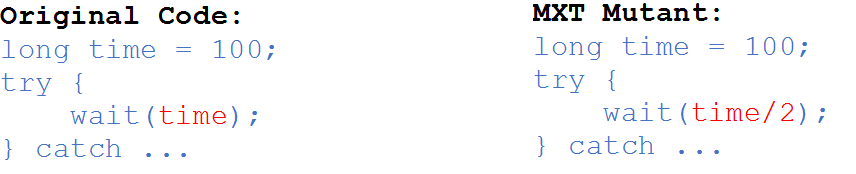
\includegraphics[scale = 0.55]{MXT.png}
    \caption{MXT mutation \citep{bradbury06}}
    \label{fig:MXT}
\end{figure}

In this example, prior to the mutation, the wait time had been set to a sufficient length to allow other threads to fully execute any concurrent operations that may interfere with mutually accessed resources. However, cutting this time in half may not leave enough time for another thread to complete execution. Various similar problems can occur when applying the MXT mutation to the other concurrent methods mentioned above. These errors will be discussed in the Results section, for each method tested.  

\subsubsection{MSP - Modify Synchronized Block Parameter}
	
The MSP is another \textit{Modify Parameters of Concurrent Method} operator that alters the parameter of a synchronized block. The \textit{synchronized} keyword is applied to an object that the programmer wishes to be thread safe when executed by blocking other concurrent actions from taking place. The mutation made by this operator aims to replace the synchronized object parameter with another object \citep{bradbury06}. The simplest method of achieving this is to replace the object with the keyword \textit{this}. An example of this is given in Figure \ref{fig:MSP}.

\begin{figure}[h]
    \centering
    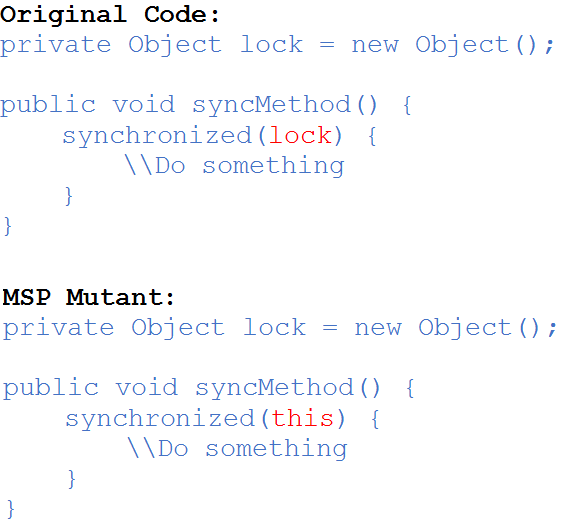
\includegraphics[scale = 0.6]{MSP.png}
    \caption{MSP mutation \citep{bradbury06}}
    \label{fig:MSP}
\end{figure}

The keyword \textit{this} refers to the current object: an instance of the class in which the method has been defined. Thus, the effects of changing the lock object to \textit{this}, the lock object becomes no longer thread safe and executing the critical section of code leaves the lock object susceptible to unpredictable behaviour when interleaving with other threads.  

\subsubsection{RTXC - Remove Thread Method-X Call}

The RTXC belongs to the \textit{Modify the Occurrence of Concurrency Method Calls} category in section \ref{section:Modify Method Calls}. This mutant simply removes calls to the Thread methods wait(), join(), sleep(), yield(), notify(), and notifyAll() \citep{bradbury06}. Figure \ref{fig:RTXC} provides an example for this mutation.

\begin{figure}[h]
    \centering
    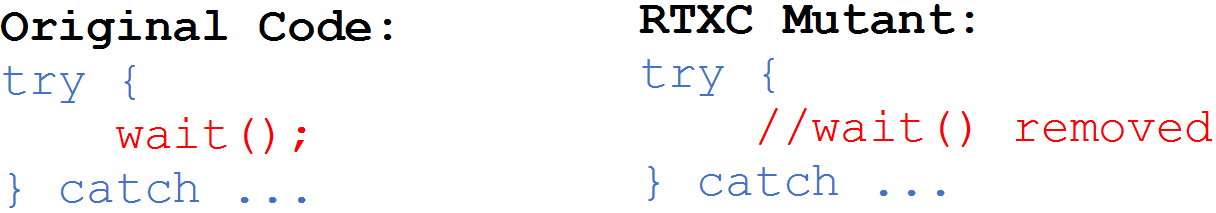
\includegraphics[scale = 0.35]{RTXC.png}
    \caption{RTXC mutation \citep{bradbury06}}
    \label{fig:RTXC}
\end{figure}

Removing a call to any of the Thread methods also removes control from the user in their ability to schedule thread execution. The behaviour of the system is likely to change from the original expectations.

\subsubsection{RCXC - Remove Concurrency Mechanism Method-X Call}

The final mutation operator that was selected aims to remove a variety of different concurrent methods: lock(), unlock(), signal(), signalAll(), acquire(), release(), countDown(), and submit() \citep{bradbury06}. It utilises the same removal mechanism as the previous operator, RTXC, and is also in the same in category, \textit{Modify the Occurrence of Concurrency Method Calls}. Potentially the most significant method removals are for the lock() and unlock() methods. This is shown in Figure \ref{fig:RCXC}. 

\begin{figure}[h]
    \centering
    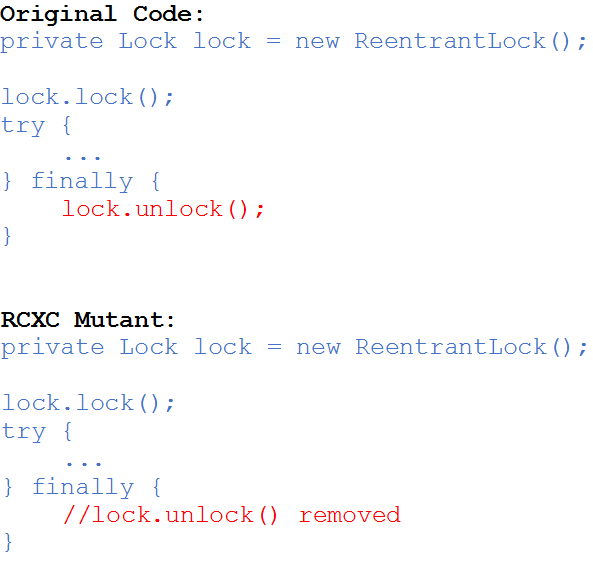
\includegraphics[scale = 0.6]{RCXC.png}
    \caption{RCXC mutation \citep{bradbury06}}
    \label{fig:RCXC}
\end{figure}	

Altering a lock on an object will have a similar behaviour to mutating a synchronized block; the object becomes no longer thread safe. Removing an unlock will prevent this thread from releasing the lock and will prevent any other threads from acquiring the lock to begin execution. Referring to work of \citet{farchi03}, this can result in a \textit{Blocking Critical Section Bug} described in section \ref{section:Blocking Code}.   
  	
	
\subsection{Mutation Tool}

With the four mutation operators identified above, the core functionality of the mutation testing tool could be designed. The main objective of the software is as follows: 

\begin{itemize}
    \item Select an input file, a mutation operator and a method to be mutated
    \item Count the number of instances of the selected method in the input file
    \item Randomly select a match and perform the mutation
    \item Write the mutation to a new file
\end{itemize}

The system consists of two classes: the Mutator class contains the methods that perform the above functionality, and the MutatorRunnable class creates a Mutator object, passes the necessary input and executes the mutation. The Mutator class accepts a File object as its only parameter. The mutation is performed by calling the replaceMutation() method.  

When running the mutation tool, the user is prompted to select an input file, an operator and a method they wish to be mutated. The tool will recognise if this combination is suitable by verifying that the input are compatible. If the user has attempted to input an incompatible pair of method and operator, then an error will flag up indicating this. This is achieved by storing a string of each operator and method in an ArrayList related to each operator. When the user inputs their desired mutation operator and method, the strings will be compared against the ArrayList contents to verify that their options are suitable. If the user selects a successful pair then the tool will begin to search the input file for any matches against the regex pattern. The matches will be returned to the user with their respective character location in the input file. The mutation is designed to only be applied to one match at random, if there are multiple matching methods. 

An algorithm was created to achieve this random selection by applying the following method. A count of the matches is stored as a local variable. The first match is encountered and a Random() function chooses a number between 1 and the count. If the random number matches the count then the first match will be selected to be mutated. The chances of this happening are 1/count; the algorithm provides an equal chance of mutation to each match. When the random number does not match, the count is reduced and the process is repeated for each subsequent match.

The following regex pattern was designed to match with any combination of mutation operator and associated method.

\begin{equation}
    \textbf{$\color{red}($}\setminus s^*.^*\setminus b \textbf{ method} \setminus (\textbf{$\color{red})($}\setminus w^*\textbf{$\color{red})($}.^*\textbf{$\color{red})$}    
\end{equation}

\noindent$ \setminus s^* $ - zero or more whitespace characters e.g. the beginning of a line
\\$ .^* $ - zero or more of any character e.g. any number of chained methods
\\$\setminus b$ - a word boundary e.g. a full stop indicating the calling of the selected method or the beginning of the line
\\$\setminus ($ - a bracket e.g. the beginning of the method parameter
\\$\setminus w*$ - zero or more of any word characters e.g. any number of parameters
\\$.*$ - zero or more of any character e.g.

The regular expression was generalised so that only one pattern was required, instead of a separate pattern for each combination of method and mutation operator. The pattern is separated into the three groups in red brackets. In general, the first group identifies the method call, the second identifies the parameters and the third identifies any syntax following the end of the parameters e.g. \textbf{)} , \textbf{\{} , \textbf{;} , etc. Before the pattern is compiled, the regex is stored as a string with the input method stored as a string variable. Thus, for any method that the user wishes to mutate, the regex string can be easily updated and then compiled as a Pattern object. Group 1 allows for the tool to easily find the specified method by the user. Group 2 is the main target for two of the mutation operators as they aim to alter the parameters. The MXT operator accesses group 2 and appends the parameter with "/2" to divide the specified length of time by 2 or simply remove the parameter altogether. The MSP operator accesses group 2 and replaces the parameter object with the keyword \textit{this}. The operators RCXC and RTXC both remove the entire method call by deleting the entire matched pattern from the code.       

Once a match has been selected, the mutation will be applied to the relevant section of code using the \textit{String.replaceFirst(regex, replacement)} method. The limitation of this method is that it will perform a replacement only on the first instance of a match within a string. To overcome this, the full input file is split into two separate strings for each match: one before, excluding the match and one after, including it. This ensures that the current selected match is the first occurrence in the second string. The mutation can therefore be applied to any of the method matches in a file. After the mutation, the two strings are stitched back together to recreate the original file with only the desired alteration. The mutant is written to a new file within the project. Note that the original file remains completely intact and the mutant is a separate file.

For example, Figure \ref{fig:rand_match} shows a code segment that has two wait methods that would match against a mutation operator such as the MXT. In this scenario, the mutation tool has identified that there are two matches. On the first iteration, when deciding which match to apply the change to, it has split the code into two strings up to the first match and after. If it decided to mutate the second match, then the two strings are shifted to before and after the second instance of wait. 

\begin{figure}[h]
    \hspace{-1.6cm}
    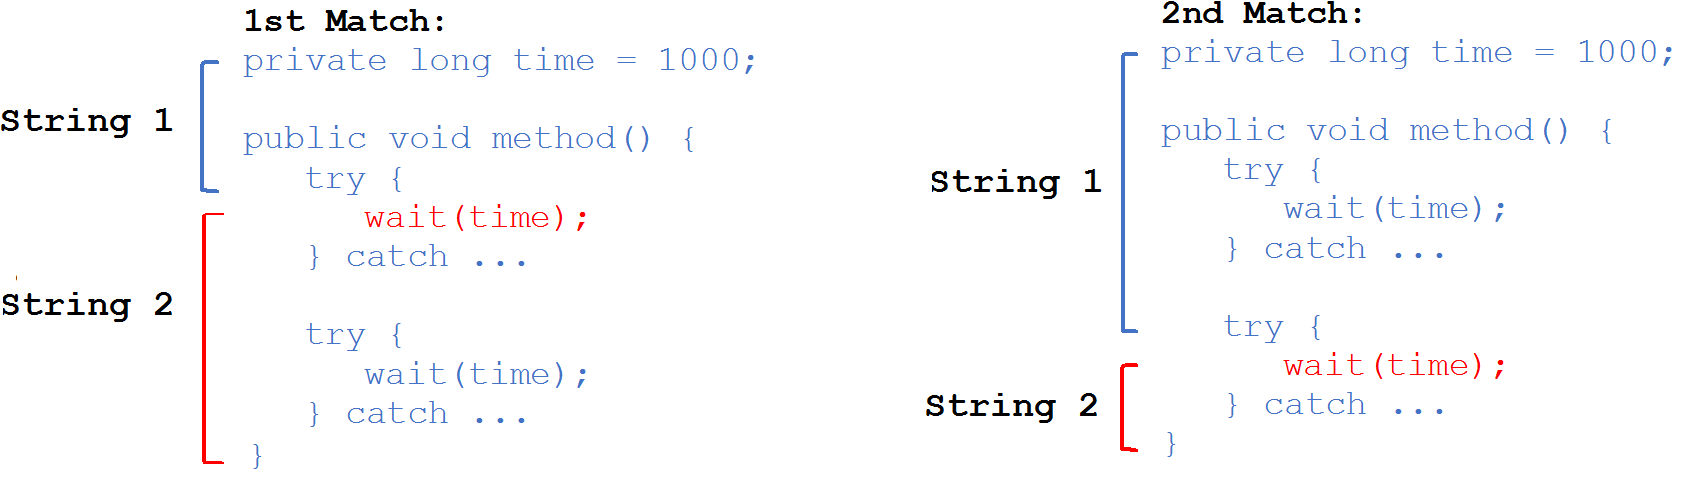
\includegraphics[scale =0.4]{random_match.png}
    \caption{Input code is split into two strings, before and after a method match.}
    \label{fig:rand_match}
\end{figure}


\subsection{Concurrent Software}

With the mutation testing tool built and the mutation operators fully implemented, to ensure the tool worked effectively, it needed some concurrent systems to test on. A typical banking system was selected after having identified that it contained a sufficient number of different concurrent features that were compatible with the four mutation operators the tool had to offer. The second, the Incrementer system, was developed to match the concurrent features found in the banking system but with different core functionality. Applying the tool to a variety of software systems provides greater verification and assurance of the tool's effectiveness. The two systems and the unit tests designed for each will be explored in detail in the following sections.


\subsubsection{Banking System}

The banking system contains four different \textit{Account} classes that provide different functionality for slightly different purposes when handling money. The \textit{Account} class is an abstract parent class that the \textit{CurrentAccount}, \textit{LoanAccount} and \textit{SavingsAccount} all inherit from. The main difference between the account classes is their specific method of withdrawing or depositing money. Each method also an associated Runnable class to allow for multi-threaded execution. The \textit{Account} class holds generic methods for depositing and transferring money, as well as the base constructor which defines the initial balance and name of the \textit{Account} object. The following methods all contain concurrent functionality in an attempt to prevent interference from interleaving threads:  \textit{deposit(double amount)}, \textit{withdraw(double amount)} and \textit{transferMoney(double amount, Account recipient)}. These methods and their functionality will be explored below. 

\textbf{\\Account - deposit(double amount)}
\\This method aims to deposit the specified amount of money into the currently accessed Account object. A lock on the critical section of code is introduced to prevent other threads from performing any interfering actions. After updating the balance, a signalAll() is called on the  concurrent condition, \textit{fundsAvailableCondition}, which informs other threads that the Account object now has a positive balance. Finally, the lock is released to allow other threads to execute concurrently.

\textbf{\\LoanAccount - deposit(double amount)}
\\The \textit{LoanAccount} overrides the parent deposit method to support the different style of account. The \textit{LoanAccount}'s purpose is to allow the user to take a loan of a specified amount of money and deposit that money into a \textit{CurrentAccount}. The initial balance of the \textit{LoanAccount} is then the negative of this amount. Money can be deposited into the \textit{LoanAccount} to pay off the loan and if the balance becomes greater than £0, the positive balance will be deposited into the \textit{CurrentAccount} from before. The deposit method utilises concurrency through the lock system and calls the parent version of the deposit method detailed above.  


\textbf{\\CurrentAccount - withdraw(double amount)}
\\The \textit{withdraw} method has the simple objective of removing money from an \textit{Account}, however, there are some rules imposed on when this is allowed. The \textit{CurrentAccount} constructor sets an overdraft limit of £50, meaning that the account cannot have less than -£50 available after any transaction. If the user attempts to withdraw an amount of money that would leave the account with less than this limit then the thread will wait until there are sufficient funds in the account by calling an \textit{await(time)} on the \textit{fundsAvailableCondition}. The thread will resume when a \textit{signal()} or\textit{ signalAll()} method is called in another thread, such as the \textit{deposit} method, or until the elapsed time has passed. In the instance of time running out and there still not being enough money in the account, the thread will be interrupted using \textit{Thread.interrupt()} and the withdrawal will not take place. After either circumstance, the method will release control of the lock it has.


\textbf{\\SavingsAccount - withdraw(double amount)}
\\The \textit{SavingsAccount} version of withdraw has the same functionality as the \textit{CurrentAccount} version with the addition of imposing a fee on each withdrawal. The user selects an amount to be withdrawn from the \textit{SavingsAccount} but this amount plus a predefined fee will be withdrawn. The concurrent features are the same as those found in the \textit{CurrentAccount} method.



\textbf{\\Account - transferMoney(double amount, Account recipient)}
\\The \textit{transferMoney} method withdraws money from one \textit{Account} and deposits that amount in another \textit{Account}, using the respective methods. Thus, it does not have any unique concurrent issues of its own, although it will encounter the same problems that can be found in the deposit and withdraw methods. A successful transfer will only take place if the withdrawal is successful and returns true.

Tables \ref{table:bank_concurrent_methods} \& \ref{table:bank_concurrent_classes} highlight every concurrent method that occurs in each of the Bank System methods described above. This information was then used to design the effective unit tests for all concurrent behaviour within the Bank System, which will be explored in Section \ref{section:Unit Tests}.


\begin{table}[]
\hspace{-2.1cm}
\begin{tabular}{lcllllll}
                                                                                                                 & \multicolumn{1}{l}{}                                                                    &                                               &                                               & \multicolumn{2}{l}{\textbf{Concurrent Feature}}                                               &                                               &                                               \\ \cline{3-8} 
                                                                                                                 & \multicolumn{1}{l|}{\textbf{}}                                                          & \multicolumn{1}{c|}{lock}                     & \multicolumn{1}{c|}{unlock}                   & \multicolumn{1}{c|}{signalAll}                & \multicolumn{1}{c|}{interrupt}                & \multicolumn{1}{c|}{await}                    & \multicolumn{1}{c|}{newCondition}             \\ \cline{2-8} 
\multicolumn{1}{l|}{}                                                                                            & \multicolumn{1}{c|}{\begin{tabular}[c]{@{}c@{}}Account \\ constructor\end{tabular}}     & \multicolumn{1}{l|}{}                         & \multicolumn{1}{l|}{}                         & \multicolumn{1}{l|}{}                         & \multicolumn{1}{l|}{}                         & \multicolumn{1}{l|}{}                         & \multicolumn{1}{l|}{\cellcolor[HTML]{32CB00}} \\ \cline{2-8} 
\multicolumn{1}{l|}{}                                                                                            & \multicolumn{1}{c|}{\begin{tabular}[c]{@{}c@{}}Account\\ deposit\end{tabular}}          & \multicolumn{1}{l|}{\cellcolor[HTML]{32CB00}} & \multicolumn{1}{l|}{\cellcolor[HTML]{32CB00}} & \multicolumn{1}{l|}{\cellcolor[HTML]{32CB00}} & \multicolumn{1}{l|}{}                         & \multicolumn{1}{l|}{}                         & \multicolumn{1}{l|}{}                         \\ \cline{2-8} 
\multicolumn{1}{c|}{}                                                                                            & \multicolumn{1}{c|}{\begin{tabular}[c]{@{}c@{}}Account\\ transferMoney\end{tabular}}    & \multicolumn{1}{l|}{\cellcolor[HTML]{32CB00}} & \multicolumn{1}{l|}{\cellcolor[HTML]{32CB00}} & \multicolumn{1}{l|}{\cellcolor[HTML]{31A4FF}} & \multicolumn{1}{l|}{\cellcolor[HTML]{31A4FF}} & \multicolumn{1}{l|}{\cellcolor[HTML]{31A4FF}} & \multicolumn{1}{l|}{}                         \\ \cline{2-8} 
\multicolumn{1}{c|}{\multirow{-2}{*}{\textbf{\begin{tabular}[c]{@{}c@{}}Bank \\ System \\ Method\end{tabular}}}} & \multicolumn{1}{c|}{\begin{tabular}[c]{@{}c@{}}LoanAccount \\ constructor\end{tabular}} & \multicolumn{1}{l|}{\cellcolor[HTML]{31A4FF}} & \multicolumn{1}{l|}{\cellcolor[HTML]{31A4FF}} & \multicolumn{1}{l|}{\cellcolor[HTML]{31A4FF}} & \multicolumn{1}{l|}{}                         & \multicolumn{1}{l|}{}                         & \multicolumn{1}{l|}{\cellcolor[HTML]{31A4FF}} \\ \cline{2-8} 
\multicolumn{1}{l|}{}                                                                                            & \multicolumn{1}{c|}{\begin{tabular}[c]{@{}c@{}}LoanAccount\\ deposit\end{tabular}}      & \multicolumn{1}{l|}{\cellcolor[HTML]{32CB00}} & \multicolumn{1}{l|}{\cellcolor[HTML]{32CB00}} & \multicolumn{1}{l|}{\cellcolor[HTML]{31A4FF}} & \multicolumn{1}{l|}{}                         & \multicolumn{1}{l|}{}                         & \multicolumn{1}{l|}{}                         \\ \cline{2-8} 
\multicolumn{1}{l|}{}                                                                                            & \multicolumn{1}{c|}{\begin{tabular}[c]{@{}c@{}}CurrentAccount\\ withdraw\end{tabular}}  & \multicolumn{1}{l|}{\cellcolor[HTML]{32CB00}} & \multicolumn{1}{l|}{\cellcolor[HTML]{32CB00}} & \multicolumn{1}{l|}{}                         & \multicolumn{1}{l|}{\cellcolor[HTML]{32CB00}} & \multicolumn{1}{l|}{\cellcolor[HTML]{32CB00}} & \multicolumn{1}{l|}{}                         \\ \cline{2-8} 
\multicolumn{1}{l|}{}                                                                                            & \multicolumn{1}{c|}{\begin{tabular}[c]{@{}c@{}}SavingsAccount\\ withdraw\end{tabular}}  & \multicolumn{1}{l|}{\cellcolor[HTML]{32CB00}} & \multicolumn{1}{l|}{\cellcolor[HTML]{32CB00}} & \multicolumn{1}{l|}{}                         & \multicolumn{1}{l|}{\cellcolor[HTML]{32CB00}} & \multicolumn{1}{l|}{\cellcolor[HTML]{32CB00}} & \multicolumn{1}{l|}{}                         \\ \cline{2-8} 
\end{tabular}
\caption{Concurrent features that occur in the Banking System methods. Green boxes indicate that the concurrent method is directly called. Blue boxes indicate that the concurrent method is indirectly called by calling another method. For example, the Account transferMoney method calls a deposit and a withdraw method which contain the concurrent methods signalAll, interrupt and await.}
\label{table:bank_concurrent_methods}
\end{table}

\begin{table}[]
\hspace{-2.1cm}
\begin{tabular}{lcllllll}
                                                                                                              & \multicolumn{1}{l}{}                &                                               &                                               & \multicolumn{2}{l}{\textbf{Concurrent Feature}}                                               &                                               &                                               \\ \cline{3-8} 
                                                                                                              & \multicolumn{1}{l|}{\textbf{}}      & \multicolumn{1}{c|}{lock}                     & \multicolumn{1}{c|}{unlock}                   & \multicolumn{1}{c|}{signalAll}                & \multicolumn{1}{c|}{interrupt}                & \multicolumn{1}{c|}{await}                    & \multicolumn{1}{c|}{newCondition}             \\ \cline{2-8} 
\multicolumn{1}{c|}{\textbf{}}                                                                                & \multicolumn{1}{c|}{Account}        & \multicolumn{1}{l|}{\cellcolor[HTML]{32CB00}} & \multicolumn{1}{l|}{\cellcolor[HTML]{32CB00}} & \multicolumn{1}{l|}{\cellcolor[HTML]{32CB00}} & \multicolumn{1}{l|}{\cellcolor[HTML]{31A4FF}} & \multicolumn{1}{l|}{\cellcolor[HTML]{31A4FF}} & \multicolumn{1}{l|}{\cellcolor[HTML]{32CB00}} \\ \cline{2-8} 
\multicolumn{1}{c|}{}                                                                                         & \multicolumn{1}{c|}{CurrentAccount} & \multicolumn{1}{l|}{\cellcolor[HTML]{32CB00}} & \multicolumn{1}{l|}{\cellcolor[HTML]{32CB00}} & \multicolumn{1}{l|}{\cellcolor[HTML]{31A4FF}} & \multicolumn{1}{l|}{\cellcolor[HTML]{32CB00}} & \multicolumn{1}{l|}{\cellcolor[HTML]{32CB00}} & \multicolumn{1}{l|}{\cellcolor[HTML]{31A4FF}} \\ \cline{2-8} 
\multicolumn{1}{c|}{\multirow{-2}{*}{\textbf{\begin{tabular}[c]{@{}c@{}}Bank\\ System\\ Class\end{tabular}}}} & \multicolumn{1}{c|}{SavingsAccount} & \multicolumn{1}{l|}{\cellcolor[HTML]{32CB00}} & \multicolumn{1}{l|}{\cellcolor[HTML]{32CB00}} & \multicolumn{1}{l|}{\cellcolor[HTML]{31A4FF}} & \multicolumn{1}{l|}{\cellcolor[HTML]{32CB00}} & \multicolumn{1}{l|}{\cellcolor[HTML]{32CB00}} & \multicolumn{1}{l|}{\cellcolor[HTML]{31A4FF}} \\ \cline{2-8} 
\multicolumn{1}{l|}{}                                                                                         & \multicolumn{1}{c|}{LoanAccount}    & \multicolumn{1}{l|}{\cellcolor[HTML]{32CB00}} & \multicolumn{1}{l|}{\cellcolor[HTML]{32CB00}} & \multicolumn{1}{l|}{\cellcolor[HTML]{31A4FF}} & \multicolumn{1}{l|}{\cellcolor[HTML]{31A4FF}} & \multicolumn{1}{l|}{\cellcolor[HTML]{31A4FF}} & \multicolumn{1}{l|}{\cellcolor[HTML]{31A4FF}} \\ \cline{2-8} 
\end{tabular}
\caption{Concurrent features that occur in the Banking System classes. Green boxes indicate that the concurrent method is directly called. Blue boxes indicate that the concurrent method is indirectly called by calling another method.}
\label{table:bank_concurrent_classes}
\end{table}


\subsubsection{Incrementer System}
The Incrementer system was designed with the specific purpose of containing all of the same concurrent features found in the Banking System. A list of these methods can be found in Tables \ref{table:incrementer_methods}. The core functionality of this system is basic and mostly involves exploiting the non-atomic action of incrementing an integer, \textit{x}, using the operation \textit{x++}. Section \ref{section:atmoic} explains this operation in detail. This system consists of one main class, Incrementer, with a variety of similar methods that perform the \textit{x++} operation but utilising different concurrent features. The motivation behind creating this system was as a proof-of-concept and to help reproduce the results of performing unit tests on the Banking System. Thus, the Incrementer system is not very complex or pertains to any practical usefulness in its functionality. Each of the Incrementer concurrent methods will be explored below.        
	    
\textbf{\\Incrementer - increment(int inc)}	    
\\The base \textit{increment} method allows the user to enter an amount to increase a global integer count by. A delay is introduced between each increment using the \textit{Thread.sleep} method. There are no safety mechanisms implemented, such as a lock or synchronized block and  the time delay was set to 750 ms to artificially provide enough time for interference to regularly occur from concurrently executing threads. This is the only concurrent feature of this method.  

\textbf{\\Incrementer - incrementLocked(int inc)}
\\The \textit{incrementLocked} method is the thread safe version of the base increment by introducing a \textit{lock} and \textit{unlock} call before and after an \textit{increment} call.  

\textbf{\\Incrementer - incrementInterrupt(int inc)}
\\This incrementing method invokes an interruption on the current thread with a \textit{Thread.interrupt()} call if the count mod 5 is equal to 0. The count will only be incremented if a \textit{Thread.interrupted()} call returns true. With unmutated code, this will always be true but applying the RTXC mutation operator on the interrupt call will cause the method to behave incorrectly.    

\textbf{\\Incrementer - incrementAwait(int inc)}
\\The \textit{incrementAwait} method operates on a similar premise to the \textit{fundsAvailableCondition} seen in the Banking System withdraw methods. This method will execute an increment if an \textit{await} call is interrupted by a \textit{signalAll}, or if the count is greater than zero at the start of execution. Otherwise, no increment will occur.

\textbf{\\Incrementer - incrementSignal(int inc)}
\\ This method is similar to the \textit{incrementLocked}, however, before releasing the lock, it will call a \textit{signalAll} on the global condition to alert the \textit{incrementAwait} method that it can continue execution. 

\textbf{\\SyncIncRunnable - run()}
\\In addition to the concurrent methods found in the Banking system, the synchronized keyword was included into the Incrementer system as it is such a key feature of concurrency and the \textit{MSP} mutation operator was implemented into the mutation tool. The \textit{SyncIncRunnable} class is separate from the \textit{Incrementer} class and is simply the mechanism by which threads can execute multiple instances of a method on the same object. The \textit{synchronized} keyword is applied to an \textit{Incrementer} object, which can be replaced with the \textit{this} keyword by the \textit{MSP} mutation. In the synchronized block, the \textit{Incrementer} object calls the basic \textit{increment} method. This will have a similar effect to calling the \textit{incrementLocked} method.  

\begin{table}[h]
\hspace{-3cm}
\scalebox{0.9}{
\begin{tabular}{cccccccccc}
\multicolumn{1}{l}{}                                                                                                  & \multicolumn{1}{l}{}                                                                   & \multicolumn{1}{l}{}                          & \multicolumn{1}{l}{}                          & \multicolumn{1}{l}{}                          & \multicolumn{3}{l}{\textbf{Concurrent Feature}}                                                                                               & \multicolumn{1}{l}{}                          & \multicolumn{1}{l}{}                          \\ \cline{3-10} 
                                                                                                                      & \multicolumn{1}{c|}{}                                                                  & \multicolumn{1}{c|}{lock}                     & \multicolumn{1}{c|}{unlock}                   & \multicolumn{1}{c|}{interrupt}                & \multicolumn{1}{c|}{signalAll}                & \multicolumn{1}{c|}{await}                    & \multicolumn{1}{c|}{newCondition}             & \multicolumn{1}{c|}{sleep}                    & \multicolumn{1}{c|}{synchronized}             \\ \cline{2-10} 
\multicolumn{1}{c|}{}                                                                                                 & \multicolumn{1}{c|}{\begin{tabular}[c]{@{}c@{}}Incrementer\\ Constructor\end{tabular}} & \multicolumn{1}{c|}{}                         & \multicolumn{1}{c|}{}                         & \multicolumn{1}{c|}{}                         & \multicolumn{1}{c|}{}                         & \multicolumn{1}{c|}{}                         & \multicolumn{1}{c|}{\cellcolor[HTML]{32CB00}} & \multicolumn{1}{c|}{}                         & \multicolumn{1}{c|}{}                         \\ \cline{2-10} 
\multicolumn{1}{c|}{}                                                                                                 & \multicolumn{1}{c|}{increment}                                                         & \multicolumn{1}{c|}{}                         & \multicolumn{1}{c|}{}                         & \multicolumn{1}{c|}{}                         & \multicolumn{1}{c|}{}                         & \multicolumn{1}{c|}{}                         & \multicolumn{1}{c|}{}                         & \multicolumn{1}{c|}{\cellcolor[HTML]{32CB00}} & \multicolumn{1}{c|}{}                         \\ \cline{2-10} 
\multicolumn{1}{c|}{}                                                                                                 & \multicolumn{1}{c|}{\begin{tabular}[c]{@{}c@{}}increment-\\ Locked\end{tabular}}       & \multicolumn{1}{c|}{\cellcolor[HTML]{32CB00}} & \multicolumn{1}{c|}{\cellcolor[HTML]{32CB00}} & \multicolumn{1}{c|}{}                         & \multicolumn{1}{c|}{}                         & \multicolumn{1}{c|}{}                         & \multicolumn{1}{c|}{}                         & \multicolumn{1}{c|}{\cellcolor[HTML]{3166FF}} & \multicolumn{1}{c|}{}                         \\ \cline{2-10} 
\multicolumn{1}{c|}{}                                                                                                 & \multicolumn{1}{c|}{\begin{tabular}[c]{@{}c@{}}increment-\\ Interrupt\end{tabular}}    & \multicolumn{1}{c|}{\cellcolor[HTML]{32CB00}} & \multicolumn{1}{c|}{\cellcolor[HTML]{32CB00}} & \multicolumn{1}{c|}{\cellcolor[HTML]{32CB00}} & \multicolumn{1}{c|}{}                         & \multicolumn{1}{c|}{}                         & \multicolumn{1}{c|}{}                         & \multicolumn{1}{c|}{\cellcolor[HTML]{3166FF}} & \multicolumn{1}{c|}{}                         \\ \cline{2-10} 
\multicolumn{1}{c|}{\multirow{-3}{*}{\textbf{\begin{tabular}[c]{@{}c@{}}Incrementer\\ System\\ Method\end{tabular}}}} & \multicolumn{1}{c|}{\begin{tabular}[c]{@{}c@{}}increment-\\ Await\end{tabular}}        & \multicolumn{1}{c|}{\cellcolor[HTML]{32CB00}} & \multicolumn{1}{c|}{\cellcolor[HTML]{32CB00}} & \multicolumn{1}{c|}{}                         & \multicolumn{1}{c|}{}                         & \multicolumn{1}{c|}{\cellcolor[HTML]{32CB00}} & \multicolumn{1}{c|}{}                         & \multicolumn{1}{c|}{\cellcolor[HTML]{3166FF}} & \multicolumn{1}{c|}{}                         \\ \cline{2-10} 
\multicolumn{1}{c|}{}                                                                                                 & \multicolumn{1}{c|}{\begin{tabular}[c]{@{}c@{}}multiplier-\\ Signal\end{tabular}}      & \multicolumn{1}{c|}{\cellcolor[HTML]{32CB00}} & \multicolumn{1}{c|}{\cellcolor[HTML]{32CB00}} & \multicolumn{1}{c|}{}                         & \multicolumn{1}{c|}{\cellcolor[HTML]{32CB00}} & \multicolumn{1}{c|}{}                         & \multicolumn{1}{c|}{}                         & \multicolumn{1}{c|}{}                         & \multicolumn{1}{c|}{}                         \\ \cline{2-10} 
\multicolumn{1}{c|}{}                                                                                                 & \multicolumn{1}{c|}{\begin{tabular}[c]{@{}c@{}}SyncInc-\\ Runnable\end{tabular}}       & \multicolumn{1}{c|}{}                         & \multicolumn{1}{c|}{}                         & \multicolumn{1}{c|}{}                         & \multicolumn{1}{c|}{}                         & \multicolumn{1}{c|}{}                         & \multicolumn{1}{c|}{}                         & \multicolumn{1}{c|}{\cellcolor[HTML]{3166FF}} & \multicolumn{1}{c|}{\cellcolor[HTML]{32CB00}} \\ \cline{2-10} 
\end{tabular}}
\caption{Concurrent features that occur in the Incrementer System methods. Green boxes indicate that the concurrent method is directly called. Blue boxes indicate that the concurrent method is indirectly called by calling another method.}
\label{table:incrementer_methods}
\end{table}


\subsection{Unit Tests} \label{section:Unit Tests}

Having identified a variety of concurrent methods and implemented operators to mutate these instances throughout a system, the next step in this project was to design effective unit tests to kill these mutations. Typically, for Java systems, the JUnit testing framework is sufficient for creating unit tests. However, JUnit lacks support for executing multiple threads concurrently and thus is not suitable for evaluating most of the software developed in this project. As a result of this, another approach to unit testing had to be taken; \textit{assert} statements provide similar functionality to that found in the JUnit framework without the same limitations relating to concurrency.

The key to writing effective unit tests is to identify each individual component of a code segment and isolate its behaviour under all possible outcomes. This involves creating tests that guarantee the execution of each different path within a method, such as the branches in an \textit{if/else} block. As well as this, it is important to observe the behaviour of a system in boundary cases where errors are most likely to arise. An example of this would be testing the statement \textit{if(x \textless y)} for each of the cases where \textit{x} is less than \textit{y}, \textit{x} is equal to \textit{y} and \textit{x} is greater than \textit{y}. Applying these principles to all sections of code will add confidence of a strong test coverage.   

Despite the limitations with concurrency discussed above, JUnit provides an extremely effective environment for testing single threaded code and ensuring that each individual component behaves as expected. A JUnit test class was created for each of the Banking system classes and the Incrementer class. All methods were tested, multiple times if they produced different outputs from varying circumstances. Even the concurrent methods were tested to ensure they behaved in the expected manner when they were executed without interaction from other threads. 

The unit tests written for concurrent actions were of a slightly different structure to the traditional unit tests using JUnit. Several scenarios were identified that could potentially lead to interfering threads attempting to access the same resource. In the Banking system, most of the methods were attempting to access and modify the balance of an Account object. If two threads attempted to deposit or withdraw money whilst another thread was modifying the balance, then the final balance query may be different from the expected value, unless the methods have the necessary precautions in place. Section \ref{section:Concurrent Bug Patterns} details the various issues that can occur when a system is not properly safeguarded from interfering threads. A total of seven concurrent unit tests were created for the Bank System and three for the Incrementer system. The two systems in their original states without mutations needed to be verified as thread-safe by passing all of their respective concurrent unit tests. These scenarios will be described below.   

\subsubsection{Banking System Concurrent Tests}

\textbf{CurrentWithdrawTest}
\\This test performs a withdrawal in one thread and a deposit in another, from a \textit{CurrentAccount}. The aim of the test is for the \textit{withdraw} to execute first and to encounter the scenario where the amount of money attempting to be withdrawn is over the limit and there is not enough money to perform the withdrawal immediately. The \textit{withdraw} thread will then wait until the account has enough money to make a successful withdrawal. Whilst this thread is interrupted, the other thread will be allowed to execute and will make a deposit to the shared \textit{CurrentAccount}. After the second thread executes a call to the \textit{signalAll} method, the first thread will resume execution and the account will have enough money available to complete the withdrawal. Without any mutations, this test should pass every time as sufficient steps have been taken to prevent any interference from the two threads.  

\textbf{\\SavingsWithdrawTest}
\\The \textit{SavingsAccount} has a near identical \textit{withdraw} method to the \textit{CurrentAccount} but with an added fee for each withdrawal. This test functions in the same manner as the \textit{CurrentWithdrawTest} above, only using the \textit{SavingsAccount} version of the \textit{withdraw} method.

\textbf{\\CurrentDoubleWithdrawTest}
\\Two withdrawals from a \textit{CurrentAccount} are attempted in this test. To pass, only one of the withdrawals can be successful, otherwise the account balance will be below the limit set on the account. The \textit{withdraw} methods makes multiple checks to the current balance before allowing a transaction to take place. However, in a thread-unsafe scenario, if one thread were to check the balance just before another thread made a successful withdrawal from the same account, then the balance it has will no longer be correct. The second thread will then be permitted to perform a second withdrawal over the limit.    

\textbf{\\SavingsDoubleWithdrawTest}
\\This repeats the above test, only using a \textit{SavingsAccount} instead of a \textit{CurrentAccount} to evaluate the \textit{withdraw} method behaviour.

\textbf{\\CurrentWithdrawLoanDepositTest}
\\This test checks that the \textit{LoanAccount deposit} method functions correctly with a corresponding \textit{CurrentAccount}. The user takes out a loan so that the \textit{CurrentAccount} initially has a positive balance and the \textit{LoanAccount} has a negative balance. The \textit{CurrentAccount} attempts to make a withdrawal that exceeds the limit and waits for funds to become available. Then a deposit will be made to the \textit{LoanAccount}, such that the balance becomes positive and the excess is deposited into the \textit{CurrentAccount} and the withdrawal from this account can proceed. For this test to pass, both methods must be functioning in a perfectly thread-safe way.   

\textbf{\\CurrentTransferTest}
\\The \textit{transfer} method moves money from one \textit{Account} to another by withdrawing from one and depositing in the other. The test for this is similar to the \textit{CurrentWithdrawTest}, where the sender attempts to transfer too much money to another account and has to wait for available funds from a deposit.  

\textbf{\\CurrentTransferDepositWithdrawTest}
\\The final test combines all of the concurrent methods in three separate threads to maximise the chances of interference. Two \textit{CurrentAccounts} are created, one sender and one receiver. The sender attempts to withdraw a large sum of money, transfer money to the other account and finally deposit a large enough sum to allow the other two transactions to be successful.  

All of these tests determine a pass or failure by evaluating the balance of each \textit{Account} object after all of the concurrent actions have taken place. The nature of the tests ensures that the outcome should always be the same for correct functionality but a mutant will likely produce a different outcome. The range of tests here covers all of the Banking system classes and all concurrent operations within them.

\subsubsection{Incrementer Concurrent Tests}

\textbf{LockTest}
\\The \textit{LockTest} performs two \textit{incrementLocked} methods in separate threads to produce the interference bug shown in Section \ref{section:atmoic} Table \ref{table:non-atomic}. Removing the locks through a mutation will mean that the threads are attempting to access and modify the \textit{Incrementer} object's count at the same time. 

\textbf{\\InterruptTest}
\\This tests the \textit{incrementInterrupt} method by calling this in one thread and an \textit{incrementLocked} in another. If the \textit{interrupt} call has been removed by a mutation, then only one set of increments will be applied to the count and the final value will not be correct. 

\textbf{\\AwaitSignalTest}
\\The \textit{AwaitSignalTest} tests for the presence of the \textit{await} and \textit{signalAll} calls in the \textit{incrementAwait} and \textit{incrementSignal} methods. The functionality of the \textit{incrementAwait} in this test, depends on the \textit{incrementSignal} to be called and release it from its interrupted waiting state. The test will always pass with unaltered code, however it will not always fail when a mutation is introduced. This is because the outcome of this scenario depends on the order in which the two threads run. Thus, this test must be run multiple times until the mutation has been veritably caught. 

Similar to the Banking system concurrent tests, the critical variable that is evaluated after concurrent actions have terminated is the count, in this case.   

\textbf{\\SyncTest}
\\This test executes two \textit{SyncIncRunnables} in separate threads with the intention of interference occurring during the increment operations. With synchronized code, the two threads will execute sequentially and will always produce the same outcome. With mutated code, the \textit{synchronized} keyword modified to \textit{this}, the code is no longer synchronized and will likely produce a different outcome every time.  


\subsection{Software Engineering Process}

IntelliJ was chosen as the IDE to develop in, utilising its intuitive layout, integration with GitHub and the various useful services it provides for refactoring and debugging. 
	
Throughout development, GitHub was used to maintain version control and keep a record of daily updates. Initially, a logbook was created and updated regularly with project development ideas; resources found during research were recorded and any useful details kept for reference. This process helped provide a structure for the project and allowed for a continual review of the software design. Once development of the software was under way and the main architectural design had been outlined, the GitHub commit messages served a similar purpose. As well as describing any changes to the code, the following steps to take in development and any problems that had been encountered were documented here. The commit messages were reviewed upon revisiting the project as a reminder of the progress.    

Aside from the concurrent unit tests written for the Banking and Incrementer systems, the mutation tool also required tests. Once a few of the mutation operators had been implemented into the tool, unit tests were created for the various methods within the Mutator class. However, as the project progressed, there became an unmanageable number of different options for each mutation operator and it was not an efficient use of time to create a unit test for each mutation. Sample files containing a small selection of the different mutable methods were created. Since many of the mutations operated on a shared mechanism of removal or parameter modification, the mutation tool was tested on only a few different methods and the outcomes were reasonably assumed to be representative of the whole selection. This method of manual observation is not necessarily as reliable as running a full suite of JUnit tests after any code modification, but the time saved during the development was worth the sacrifice.   

Each file in the concurrent systems was stored outside of the IntelliJ project, isolated from the mutation testing tool. These files were intact and contained no errors or mutations; the mutation tool would accept these clean files as input before corrupting them with mutations. After applying the mutation, unit tests had to be performed on the new file, thus each mutant had to overwrite the previous mutation and then introduce the file to the IntelliJ project where the unit tests were stored. This method ensured that the original files remained intact and that only one mutation would be present in the project version. Simultaneously, each mutation was saved to another location on file to keep a record of results.


\newpage	
\section{Analysis}
\subsection{Results}

For a test to be considered successful at killing a mutation, the outcome of the test must go from passing when applied to clean, unaltered code, to failing when applied to mutated code. The test resulting in a failure indicates that the test has identified that the behaviour of the system has changed due to the mutation i.e. the test has fulfilled its purpose. 

Since it can be difficult to predict the scheduling order of concurrently running threads, all concurrent tests were run many times until the desired result was observed. If the test managed to catch a bug in at least one of the runs then it was deemed successful, regardless of whether other runs failed to kill a mutation. For each mutation, all of the tests relating to the mutated file were run and the result of a mutation surviving or not was assessed across the whole range of tests. If one of the tests reported the presence of a mutation but the others did not, the mutation would still be deemed to have been successfully killed.

The results of the tests will be displayed in sections \ref{section:Banking System Results} \& \ref{section:Incrementer System Results}, where green results indicate that a mutation was successfully killed i.e. the test returned with a failure. Red indicates that a mutation went undiscovered i.e. the test returned with a pass. Blue indicates that some other error occurred e.g. a compilation error prevented the test from running. The JUnit tests have a slight variation in what is considered a test failure compared to the concurrent tests. JUnit tests can produce a failure when the observed state of the variables after execution are in accordance with the expected outcome, such as a correct account balance, but if an \textit{IllegalMonitorStateException} is thrown, for example, then the test will not pass despite the methods otherwise functioning properly. In opposition, determining a failure for the concurrent tests relies purely on the outcome of the various account balances and exceptions are treated as blue results. The reason for the separate definitions is to differentiate between a failed test due to a behavioural change that caused the system to result in a different state to the expected, as opposed to an error thrown but the system still managed to result in the correct final balance. For all intents and purposes, a blue result can be considered to have killed a mutation as the error produced indicates to the user that the system is not working perfectly. 
The two most common types of exceptions that are thrown from a mutation that will produce a blue result for concurrent tests, are the \textit{IllegalMonitorStateException} and the \textit{NullPointerException}. 

\begin{description}
    \item[\textbf{IllegalMonitorStateException -}]API description: \textit{"Thrown to indicate that a thread has attempted to wait on an object's monitor or to notify other threads waiting on an object's monitor without owning the specified monitor."} \citep{imse18}. This typically occurs when removing a \textit{lock} method whilst leaving the corresponding \textit{unlock} method intact. The error is thrown because the command to release the object's lock on the monitor is given, even though the object never obtained the lock in the first place, due to the mutation. 

    \item[\textbf{NullPointerException - }] API description: \textit{"Thrown when an application attempts to use null in a case where an object is required."} \citep{npe18}. A very familiar error to any Java developer, although, specifically in these tests, this error is almost exclusively thrown when removing a \textit{newCondition}. Removing this method declaration in the \textit{Incrementer} constructor consequently means that when the \textit{withdraw} method attempts to call an \textit{await} on the \textit{fundsAvailableCondition}, the condition does not exist, hence the method is attempting to use null instead of an object.  
\end{description}

A mutation test score will be provided for each results table and a combined score for the whole system. The mutation test score is a ratio of mutants killed to the total number of mutants tested, expressed as a percentage. One score will be given excluding blue results and one including them, the latter being the more significant value. 

\subsubsection{Banking System Results} \label{section:Banking System Results}

The results for all concurrent and JUnit tests for the Banking system are displayed in Tables \ref{table:banking_junit_results}-\ref{table:banking_combined_results}. 

\newpage
\begin{table}[htp]
\hspace{-1cm}
\begin{tabular}{lcllllll}
                                                                                        & \textbf{JUnit}                                                                                 &                                               &                                               \\
                                                                                                                 & \multicolumn{1}{l}{}           &                                               &                                               & \multicolumn{2}{l}{\textbf{Concurrent Feature}}                                               &                                               &                                               \\ \cline{3-8} 
                                                                                                                 & \multicolumn{1}{l|}{\textbf{}} & \multicolumn{1}{c|}{lock}                     & \multicolumn{1}{c|}{unlock}                   & \multicolumn{1}{c|}{signalAll}                & \multicolumn{1}{c|}{interrupt}                & \multicolumn{1}{c|}{await}                    & \multicolumn{1}{c|}{newCondition}             \\ \cline{2-8} 
\multicolumn{1}{l|}{}                                                                                            & \multicolumn{1}{c|}{Account}   & \multicolumn{1}{l|}{\cellcolor[HTML]{32CB00}} & \multicolumn{1}{l|}{\cellcolor[HTML]{32CB00}} & \multicolumn{1}{l|}{\cellcolor[HTML]{FE0000}} & \multicolumn{1}{l|}{\cellcolor[HTML]{FFFFFF}} & \multicolumn{1}{l|}{\cellcolor[HTML]{FFFFFF}} & \multicolumn{1}{l|}{\cellcolor[HTML]{32CB00}} \\ \cline{2-8} 
\multicolumn{1}{c|}{}                                                                                            & \multicolumn{1}{c|}{Current}   & \multicolumn{1}{l|}{\cellcolor[HTML]{32CB00}} & \multicolumn{1}{l|}{\cellcolor[HTML]{FE0000}} & \multicolumn{1}{l|}{\cellcolor[HTML]{FFFFFF}} & \multicolumn{1}{l|}{\cellcolor[HTML]{32CB00}} & \multicolumn{1}{l|}{\cellcolor[HTML]{31A4FF}} & \multicolumn{1}{l|}{\cellcolor[HTML]{FFFFFF}} \\ \cline{2-8} 
\multicolumn{1}{c|}{\multirow{-2}{*}{\textbf{\begin{tabular}[c]{@{}c@{}}Banking\\ System\\ Class\end{tabular}}}} & \multicolumn{1}{c|}{Loan}      & \multicolumn{1}{l|}{\cellcolor[HTML]{32CB00}} & \multicolumn{1}{l|}{\cellcolor[HTML]{FE0000}} & \multicolumn{1}{l|}{\cellcolor[HTML]{FFFFFF}} & \multicolumn{1}{l|}{\cellcolor[HTML]{FFFFFF}} & \multicolumn{1}{l|}{\cellcolor[HTML]{FFFFFF}} & \multicolumn{1}{l|}{\cellcolor[HTML]{FFFFFF}} \\ \cline{2-8} 
\multicolumn{1}{c|}{\textbf{}}                                                                                   & \multicolumn{1}{c|}{Savings}   & \multicolumn{1}{l|}{\cellcolor[HTML]{32CB00}} & \multicolumn{1}{l|}{\cellcolor[HTML]{FE0000}} & \multicolumn{1}{l|}{\cellcolor[HTML]{FFFFFF}} & \multicolumn{1}{l|}{\cellcolor[HTML]{32CB00}} & \multicolumn{1}{l|}{\cellcolor[HTML]{31A4FF}} & \multicolumn{1}{l|}{\cellcolor[HTML]{FFFFFF}} \\ \cline{2-8} 
\end{tabular}
\caption{JUnit test results for mutations applied to the selected concurrent methods in each of the Banking system classes. Mutation test score excluding blue results: 57\%. Score including blue results: 71\%}
\label{table:banking_junit_results}
\end{table}

\vspace{3cm}

\begin{table}[hp!]
\hspace{-1cm}
\begin{tabular}{lcllll}
                                                                                        & \multicolumn{1}{l}{\textbf{Account}}                                                             &                                               &                                               &                                               &                                               \\
                                                                                        & \multicolumn{1}{l}{}                                                                             &                                               & \multicolumn{2}{l}{\textbf{Concurrent Feature}}                                               &                                               \\ \cline{3-6} 
                                                                                        & \multicolumn{1}{l|}{\textbf{}}                                                                   & \multicolumn{1}{c|}{lock}                     & \multicolumn{1}{c|}{unlock}                   & \multicolumn{1}{c|}{signalAll}                & \multicolumn{1}{c|}{newCondition}             \\ \cline{2-6} 
\multicolumn{1}{l|}{}                                                                   & \multicolumn{1}{c|}{\begin{tabular}[c]{@{}c@{}}Current\\ Withdraw\end{tabular}}                  & \multicolumn{1}{l|}{\cellcolor[HTML]{31A4FF}} & \multicolumn{1}{l|}{\cellcolor[HTML]{32CB00}} & \multicolumn{1}{l|}{\cellcolor[HTML]{FE0000}} & \multicolumn{1}{l|}{\cellcolor[HTML]{32CB00}} \\ \cline{2-6} 
\multicolumn{1}{c|}{\textbf{}}                                                          & \multicolumn{1}{c|}{\begin{tabular}[c]{@{}c@{}}Savings\\ Withdraw\end{tabular}}                  & \multicolumn{1}{l|}{\cellcolor[HTML]{31A4FF}} & \multicolumn{1}{l|}{\cellcolor[HTML]{32CB00}} & \multicolumn{1}{l|}{\cellcolor[HTML]{FE0000}} & \multicolumn{1}{l|}{\cellcolor[HTML]{31A4FF}} \\ \cline{2-6} 
\multicolumn{1}{c|}{\textbf{\begin{tabular}[c]{@{}c@{}}Concurrent\\ Test\end{tabular}}} & \multicolumn{1}{c|}{\begin{tabular}[c]{@{}c@{}}Current Transfer\\ Deposit\end{tabular}}          & \multicolumn{1}{l|}{\cellcolor[HTML]{31A4FF}} & \multicolumn{1}{l|}{\cellcolor[HTML]{32CB00}} & \multicolumn{1}{l|}{\cellcolor[HTML]{FE0000}} & \multicolumn{1}{l|}{\cellcolor[HTML]{31A4FF}} \\ \cline{2-6} 
\multicolumn{1}{c|}{\textbf{}}                                                          & \multicolumn{1}{c|}{\begin{tabular}[c]{@{}c@{}}Current Transfer\\ Deposit Withdraw\end{tabular}} & \multicolumn{1}{l|}{\cellcolor[HTML]{31A4FF}} & \multicolumn{1}{l|}{\cellcolor[HTML]{32CB00}} & \multicolumn{1}{l|}{\cellcolor[HTML]{FE0000}} & \multicolumn{1}{l|}{\cellcolor[HTML]{31A4FF}} \\ \cline{2-6} 
\multicolumn{1}{l|}{}                                                                   & \multicolumn{1}{c|}{\begin{tabular}[c]{@{}c@{}}Current Withdraw\\ Loan Deposit\end{tabular}}     & \multicolumn{1}{l|}{\cellcolor[HTML]{31A4FF}} & \multicolumn{1}{l|}{\cellcolor[HTML]{32CB00}} & \multicolumn{1}{l|}{\cellcolor[HTML]{FE0000}} & \multicolumn{1}{l|}{\cellcolor[HTML]{31A4FF}} \\ \cline{2-6} 
\end{tabular}
\caption{Results of concurrent tests for mutations applied to the \textit{Account} class. Mutation test score excluding blue results: 50\%. Score including blue results: 75\%}
\label{table:account_results}
\end{table}

\begin{table}[hp!]
\begin{tabular}{lcllll}
                                                                                        & \multicolumn{1}{l}{\textbf{Current}}                                                             &                                               &                                               &                                               &                                               \\
                                                                                        & \multicolumn{1}{l}{}                                                                             &                                               & \multicolumn{2}{l}{\textbf{Concurrent Feature}}                                               &                                               \\ \cline{3-6} 
                                                                                        & \multicolumn{1}{l|}{\textbf{}}                                                                   & \multicolumn{1}{c|}{lock}                     & \multicolumn{1}{c|}{unlock}                   & \multicolumn{1}{c|}{interrupt}                & \multicolumn{1}{c|}{await}                    \\ \cline{2-6} 
\multicolumn{1}{l|}{}                                                                   & \multicolumn{1}{c|}{\begin{tabular}[c]{@{}c@{}}Current\\ Withdraw\end{tabular}}                  & \multicolumn{1}{l|}{\cellcolor[HTML]{31A4FF}} & \multicolumn{1}{l|}{\cellcolor[HTML]{FE0000}} & \multicolumn{1}{l|}{\cellcolor[HTML]{FE0000}} & \multicolumn{1}{l|}{\cellcolor[HTML]{31A4FF}} \\ \cline{2-6} 
\multicolumn{1}{c|}{\textbf{}}                                                          & \multicolumn{1}{c|}{\begin{tabular}[c]{@{}c@{}}Current Double\\ Withdraw\end{tabular}}           & \multicolumn{1}{l|}{\cellcolor[HTML]{31A4FF}} & \multicolumn{1}{l|}{\cellcolor[HTML]{32CB00}} & \multicolumn{1}{l|}{\cellcolor[HTML]{32CB00}} & \multicolumn{1}{l|}{\cellcolor[HTML]{31A4FF}} \\ \cline{2-6} 
\multicolumn{1}{c|}{\textbf{\begin{tabular}[c]{@{}c@{}}Concurrent\\ Test\end{tabular}}} & \multicolumn{1}{c|}{\begin{tabular}[c]{@{}c@{}}Current Transfer\\ Deposit\end{tabular}}          & \multicolumn{1}{l|}{\cellcolor[HTML]{31A4FF}} & \multicolumn{1}{l|}{\cellcolor[HTML]{FE0000}} & \multicolumn{1}{l|}{\cellcolor[HTML]{FE0000}} & \multicolumn{1}{l|}{\cellcolor[HTML]{31A4FF}} \\ \cline{2-6} 
\multicolumn{1}{c|}{\textbf{}}                                                          & \multicolumn{1}{c|}{\begin{tabular}[c]{@{}c@{}}Current Transfer\\ Deposit Withdraw\end{tabular}} & \multicolumn{1}{l|}{\cellcolor[HTML]{31A4FF}} & \multicolumn{1}{l|}{\cellcolor[HTML]{32CB00}} & \multicolumn{1}{l|}{\cellcolor[HTML]{FE0000}} & \multicolumn{1}{l|}{\cellcolor[HTML]{31A4FF}} \\ \cline{2-6} 
\multicolumn{1}{l|}{}                                                                   & \multicolumn{1}{c|}{\begin{tabular}[c]{@{}c@{}}Current Withdraw\\ Loan Deposit\end{tabular}}     & \multicolumn{1}{l|}{\cellcolor[HTML]{32CB00}} & \multicolumn{1}{l|}{\cellcolor[HTML]{FE0000}} & \multicolumn{1}{l|}{\cellcolor[HTML]{FE0000}} & \multicolumn{1}{l|}{\cellcolor[HTML]{31A4FF}} \\ \cline{2-6} 
\end{tabular}
\caption{Results of concurrent tests for mutations applied to the \textit{CurrentAccount} class. Mutation test score excluding blue results: 75\%. Score including blue results: 100\%}
\label{table:current_results}
\end{table}

\begin{table}[hp!]
\begin{tabular}{llllll}
                                                                                        & \textbf{Savings}                                                                       &                                               &                                               &                                               &                                               \\
                                                                                        &                                                                                        &                                               & \multicolumn{2}{l}{\textbf{Concurrent Feature}}                                               &                                               \\ \cline{3-6} 
                                                                                        & \multicolumn{1}{l|}{\textbf{}}                                                         & \multicolumn{1}{c|}{lock}                     & \multicolumn{1}{c|}{unlock}                   & \multicolumn{1}{c|}{interrupt}                & \multicolumn{1}{c|}{await}                    \\ \cline{2-6} 
\multicolumn{1}{c|}{\textbf{\begin{tabular}[c]{@{}c@{}}Concurrent\\ Test\end{tabular}}} & \multicolumn{1}{c|}{\begin{tabular}[c]{@{}c@{}}Savings\\ Withdraw\end{tabular}}        & \multicolumn{1}{l|}{\cellcolor[HTML]{31A4FF}} & \multicolumn{1}{l|}{\cellcolor[HTML]{FE0000}} & \multicolumn{1}{l|}{\cellcolor[HTML]{FE0000}} & \multicolumn{1}{l|}{\cellcolor[HTML]{31A4FF}} \\ \cline{2-6} 
\multicolumn{1}{c|}{\textbf{}}                                                          & \multicolumn{1}{c|}{\begin{tabular}[c]{@{}c@{}}Savings Double\\ Withdraw\end{tabular}} & \multicolumn{1}{l|}{\cellcolor[HTML]{31A4FF}} & \multicolumn{1}{l|}{\cellcolor[HTML]{32CB00}} & \multicolumn{1}{l|}{\cellcolor[HTML]{32CB00}} & \multicolumn{1}{l|}{\cellcolor[HTML]{31A4FF}} \\ \cline{2-6} 
\end{tabular}
\caption{Results of concurrent tests for mutations applied to the \textit{SavingsAccount} class. Mutation test score excluding blue results: 50\%. Score including blue results: 100\%}
\label{table:savings_results}
\end{table}

\begin{table}[hp!]
\begin{tabular}{llll}
                                                                                        & \textbf{Loan}                                                                                &                                               &                                               \\
                                                                                        &                                                                                              & \multicolumn{2}{c}{\textbf{Concurrent Feature}}                                               \\ \cline{3-4} 
                                                                                        & \multicolumn{1}{l|}{\textbf{}}                                                               & \multicolumn{1}{c|}{lock}                     & \multicolumn{1}{c|}{unlock}                   \\ \cline{2-4} 
\multicolumn{1}{c|}{\textbf{\begin{tabular}[c]{@{}c@{}}Concurrent\\ Test\end{tabular}}} & \multicolumn{1}{c|}{\begin{tabular}[c]{@{}c@{}}Current Withdraw\\ Loan Deposit\end{tabular}} & \multicolumn{1}{l|}{\cellcolor[HTML]{31A4FF}} & \multicolumn{1}{l|}{\cellcolor[HTML]{FE0000}} \\ \cline{2-4} 
\end{tabular}
\caption{Results of concurrent tests for mutations applied to the \textit{LoanAccount} class. Mutation test score excluding blue results: 0\%. Score including blue results: 50\%.}
\label{table:loan_results}
\end{table}

\begin{table}[hp!]
\hspace{-1cm}
\begin{tabular}{lcllllll}
                                                                                        & \textbf{All Classes}                                                                                 &                                               &                                               \\
                                                                                                                 & \multicolumn{1}{l}{}           &                                               &                                               & \multicolumn{2}{l}{\textbf{Concurrent Feature}}                                               &                                               &                                               \\ \cline{3-8} 
                                                                                                                 & \multicolumn{1}{l|}{\textbf{}} & \multicolumn{1}{c|}{lock}                     & \multicolumn{1}{c|}{unlock}                   & \multicolumn{1}{c|}{signalAll}                & \multicolumn{1}{c|}{interrupt}                & \multicolumn{1}{c|}{await}                    & \multicolumn{1}{c|}{newCondition}             \\ \cline{2-8} 
\multicolumn{1}{l|}{}                                                                                            & \multicolumn{1}{c|}{Account}   & \multicolumn{1}{l|}{\cellcolor[HTML]{31A4FF}} & \multicolumn{1}{l|}{\cellcolor[HTML]{32CB00}} & \multicolumn{1}{l|}{\cellcolor[HTML]{FE0000}} & \multicolumn{1}{l|}{\cellcolor[HTML]{FFFFFF}} & \multicolumn{1}{l|}{\cellcolor[HTML]{FFFFFF}} & \multicolumn{1}{l|}{\cellcolor[HTML]{32CB00}} \\ \cline{2-8} 
\multicolumn{1}{c|}{}                                                                                            & \multicolumn{1}{c|}{Current}   & \multicolumn{1}{l|}{\cellcolor[HTML]{32CB00}} & \multicolumn{1}{l|}{\cellcolor[HTML]{32CB00}} & \multicolumn{1}{l|}{\cellcolor[HTML]{FFFFFF}} & \multicolumn{1}{l|}{\cellcolor[HTML]{32CB00}} & \multicolumn{1}{l|}{\cellcolor[HTML]{31A4FF}} & \multicolumn{1}{l|}{\cellcolor[HTML]{FFFFFF}} \\ \cline{2-8} 
\multicolumn{1}{c|}{\multirow{-2}{*}{\textbf{\begin{tabular}[c]{@{}c@{}}Banking\\ System\\ Class\end{tabular}}}} & \multicolumn{1}{c|}{Loan}      & \multicolumn{1}{l|}{\cellcolor[HTML]{31A4FF}} & \multicolumn{1}{l|}{\cellcolor[HTML]{FE0000}} & \multicolumn{1}{l|}{\cellcolor[HTML]{FFFFFF}} & \multicolumn{1}{l|}{\cellcolor[HTML]{FFFFFF}} & \multicolumn{1}{l|}{\cellcolor[HTML]{FFFFFF}} & \multicolumn{1}{l|}{\cellcolor[HTML]{FFFFFF}} \\ \cline{2-8} 
\multicolumn{1}{c|}{\textbf{}}                                                                                   & \multicolumn{1}{c|}{Savings}   & \multicolumn{1}{l|}{\cellcolor[HTML]{31A4FF}} & \multicolumn{1}{l|}{\cellcolor[HTML]{32CB00}} & \multicolumn{1}{l|}{\cellcolor[HTML]{FFFFFF}} & \multicolumn{1}{l|}{\cellcolor[HTML]{32CB00}} & \multicolumn{1}{l|}{\cellcolor[HTML]{31A4FF}} & \multicolumn{1}{l|}{\cellcolor[HTML]{FFFFFF}} \\ \cline{2-8} 
\end{tabular}
\caption{Concurrent test results for mutations applied to the selected concurrent methods in each of the Banking system classes. Mutation test score excluding blue results: 50\%. Score including blue results: 86\%.}
\label{table:banking_all_classes_results}
\end{table}

\begin{table}[hp!]
\hspace{-1cm}
\begin{tabular}{lcllllll}
                                                                                                                 & \multicolumn{3}{l}{\textbf{Combined Results}}                                                                                  &                                               &                                               &                                               &                                               \\
                                                                                                                 & \multicolumn{1}{l}{}           & \multicolumn{1}{c}{\textbf{}}                 & \textbf{}                                     & \multicolumn{2}{c}{\textbf{Concurrent Feature}}                                               &                                               &                                               \\ \cline{3-8} 
                                                                                                                 & \multicolumn{1}{l|}{\textbf{}} & \multicolumn{1}{c|}{lock}                     & \multicolumn{1}{c|}{unlock}                   & \multicolumn{1}{c|}{signalAll}                & \multicolumn{1}{c|}{interrupt}                & \multicolumn{1}{c|}{await}                    & \multicolumn{1}{c|}{newCondition}             \\ \cline{2-8} 
\multicolumn{1}{c|}{\textbf{}}                                                                                   & \multicolumn{1}{c|}{Account}   & \multicolumn{1}{l|}{\cellcolor[HTML]{32CB00}} & \multicolumn{1}{l|}{\cellcolor[HTML]{32CB00}} & \multicolumn{1}{l|}{\cellcolor[HTML]{FE0000}} & \multicolumn{1}{l|}{}                         & \multicolumn{1}{l|}{}                         & \multicolumn{1}{l|}{\cellcolor[HTML]{32CB00}} \\ \cline{2-8} 
\multicolumn{1}{c|}{}                                                                                            & \multicolumn{1}{c|}{Current}   & \multicolumn{1}{l|}{\cellcolor[HTML]{32CB00}} & \multicolumn{1}{l|}{\cellcolor[HTML]{32CB00}} & \multicolumn{1}{l|}{}                         & \multicolumn{1}{l|}{\cellcolor[HTML]{32CB00}} & \multicolumn{1}{l|}{\cellcolor[HTML]{31A4FF}} & \multicolumn{1}{l|}{}                         \\ \cline{2-8} 
\multicolumn{1}{c|}{\multirow{-2}{*}{\textbf{\begin{tabular}[c]{@{}c@{}}Banking\\ System\\ Class\end{tabular}}}} & \multicolumn{1}{c|}{Loan}      & \multicolumn{1}{l|}{\cellcolor[HTML]{32CB00}} & \multicolumn{1}{l|}{\cellcolor[HTML]{FE0000}} & \multicolumn{1}{l|}{}                         & \multicolumn{1}{l|}{}                         & \multicolumn{1}{l|}{}                         & \multicolumn{1}{l|}{}                         \\ \cline{2-8} 
\multicolumn{1}{l|}{}                                                                                            & \multicolumn{1}{c|}{Savings}   & \multicolumn{1}{l|}{\cellcolor[HTML]{32CB00}} & \multicolumn{1}{l|}{\cellcolor[HTML]{32CB00}} & \multicolumn{1}{l|}{}                         & \multicolumn{1}{l|}{\cellcolor[HTML]{32CB00}} & \multicolumn{1}{l|}{\cellcolor[HTML]{31A4FF}} & \multicolumn{1}{l|}{}                         \\ \cline{2-8} 
\end{tabular}
\caption{Combined test results for the Banking system JUnit tests and Concurrent Tests. Mutation test score excluding blue results: 71\%. Score including blue results: 86\%.}
\label{table:banking_combined_results}
\end{table}

\newpage
The most surprising finding from the results is how well the JUnit tests performed at identifying mutations without having to run multiple threads. Comparing the mutation test scores of the JUnit tests with the concurrent tests, the JUnit tests outperformed the concurrent ones for the scores excluding blue results - 57\% to 50\%, respectively found in Tables \ref{table:banking_junit_results} \& \ref{table:banking_all_classes_results}.  

The concurrent tests have proven to be very effective when including the errors from the blue results, reaching a mutation score of 86\% which matches that of the combined results with the JUnit tests. This could indicate that the JUnit tests are superfluous, as they do not kill any additional mutants to the concurrent ones. Although, from a development point of view, JUnit tests are quick and easy to produce and can provide instant feedback for many concurrent bugs in a system without having to design bespoke tests for each concurrency issue that can occur. JUnit tests are also extremely useful for ensuring that the basic functionality of methods function in the expected manner, whereas the concurrent tests are more representative of the actual use of the system and confirm the robustness of handling issues. The ideal testing suite would utilise JUnit and concurrent tests to reap the benefits of both styles.

For the case of the \textit{await} statements in the \textit{CurrentAccount} and \textit{SavingsAccount withdraw} method, any mutation applied to it produced an \textit{InterruptedException} error that prohibited compilation. The \textit{await} statement requires a corresponding catch block for the \textit{InterruptedException}, but removing the statement leaves the try block empty of any functionality that will produce an interruption. Consequently, no test was able to run after this mutation, although the mutation can be considered to have been killed as the user would become aware of the error when attempting to compile the code. Comparing to the Pitest tool's definitions in section \ref{section:Mutation Testing}, this would be considered a 'run error' result, but within the realms of this project, it will be considered a successful catch. 

The \textit{RCXC} mutation operator removing the \textit{lock} method, always produced an \textit{IllegalMonitorStateException}. JUnit tests flag this as a failure, and although the concurrent tests reported the same exception, executing the code produced the same outcome as the pre-mutated version of the code, so it is reported as a blue result in Tables \ref{table:account_results}-\ref{table:banking_all_classes_results}.

When catching the mutations that removed the \textit{unlock} and \textit{interrupt} methods, executing the code would cause the system to hang and the threads would never achieve termination. For the \textit{unlock}, this occurs because whichever thread executes first and obtains the lock on the monitor would never release the lock to allow the other thread to begin execution. Referring to bug patterns identified by \citet{bradbury06}, this is an example of a 'blocking critical section' bug, which is defined in section \ref{section:Blocking Code}.     

For the removal of the \textit{fundsAvailableCondition} instantiation with \textit{newCondition} in the \textit{Account} class, a \textit{NullPointerException} was thrown, which resulted in the blue results seen in Table \ref{table:account_results}. However, the \textit{CurrentWithdraw} test did manage to kill the mutation by observing an unexpected account balance value.  

\subsubsection{Incrementer System Results} \label{section:Incrementer System Results} 

The results for all JUnit and concurrent tests for the \textit{Incrementer} system are displayed in Tables \ref{table:inc_junit_results} \& \ref{table:inc_concurrent_results}. Since the concurrent tests managed to kill all of the mutations, the combined results of the JUnit and concurrent tests are the same as just the concurrent test results.

Compared to the \textit{Banking} system, the JUnit tests have been significantly less successful with lower mutation scores excluding blue results, 57\% compared to 46\%, and more notably, including the blue results, 71\% compared to 54\% (Tables \ref{table:banking_junit_results} \& \ref{table:inc_junit_results}). The concurrent tests, however, were extremely effective at killing mutations and significantly outperformed the \textit{Banking} system: 50\% compared to 91\% excluding blue results and 86\% compared to 100\% including blue results, respectively (Tables \ref{table:banking_all_classes_results} \& \ref{table:inc_concurrent_results}). Finally, the combined results also noted an improvement from the \textit{Banking} system: 71\% to 92\% and 86\% to 100\%, excluding and including blue results, respectively (Tables \ref{table:banking_combined_results} \& \ref{table:inc_concurrent_results}). Initially this may seem surprising that both style of tests did not follow the same trend of either being more or less successful with respect to the other \textit{Banking} system. However, this is likely due to the overall design of the two systems serving different purposes. The \textit{Banking} system was designed to be a useful piece of software and had specific functional requirements to meet. It is larger and more complex than the \textit{Incrementer} system, with multiple different interacting methods across a range of classes. On the other hand, the \textit{Incrementer} system functionality was not designed to serve a useful purpose to the user. Instead, the methods were designed with a focus on the concurrent tests and discovering the most simple procedures that could be tested with ease. The complexity of the \textit{Banking} system consequently means that various methods are co-dependent on each other and more noticeable problems likely to arise when introducing a mutation. This produced small domino effects on the dependent methods that allowed the JUnit tests a greater opportunity to identify faults in the code, without having to utilise multiple threads. In contrast, the \textit{Incrementer} system's simple design with independent methods means that altering concurrent features has little to no effect on single threaded execution, but dramatic effects on multi-threaded execution. 


\begin{table}[hp!]
\hspace{-2.9cm}
\begin{tabular}{ccccccccc}
\multicolumn{1}{l}{}                                                                                                      & \multicolumn{3}{l}{\textbf{JUnit Tests}}                                                                                                                                               & \multicolumn{1}{l}{}                          & \multicolumn{1}{l}{}                          & \multicolumn{1}{l}{}                          & \multicolumn{1}{l}{}                          & \multicolumn{1}{l}{}                          \\
\multicolumn{1}{l}{}                                                                                                      & \multicolumn{1}{l}{}                                                                   & \multicolumn{1}{l}{}                          & \multicolumn{1}{l}{}                          & \multicolumn{1}{l}{}                        & \multicolumn{3}{l}{\textbf{Concurrent Feature}}                                                                                               & \multicolumn{1}{l}{}                          \\ \cline{3-9} 
                                                                                                                          & \multicolumn{1}{c|}{}                                                                  & \multicolumn{1}{c|}{lock}                     & \multicolumn{1}{c|}{unlock}                   & \multicolumn{1}{c|}{interrupt}                & \multicolumn{1}{c|}{signalAll}                & \multicolumn{1}{c|}{await}                    & \multicolumn{1}{c|}{newCondition}             & \multicolumn{1}{c|}{synchronized}             \\ \cline{2-9} 
\multicolumn{1}{c|}{}                                                                                                     & \multicolumn{1}{c|}{\begin{tabular}[c]{@{}c@{}}Incrementer\\ constructor\end{tabular}} & \multicolumn{1}{c|}{}                         & \multicolumn{1}{c|}{}                         & \multicolumn{1}{c|}{}                         & \multicolumn{1}{c|}{}                         & \multicolumn{1}{c|}{}                         & \multicolumn{1}{c|}{\cellcolor[HTML]{32CB00}} & \multicolumn{1}{c|}{}                         \\ \cline{2-9} 
\multicolumn{1}{c|}{\textbf{}}                                                                                            & \multicolumn{1}{c|}{\begin{tabular}[c]{@{}c@{}}increment-\\ Locked\end{tabular}}       & \multicolumn{1}{c|}{\cellcolor[HTML]{32CB00}} & \multicolumn{1}{c|}{\cellcolor[HTML]{FE0000}} & \multicolumn{1}{c|}{}                         & \multicolumn{1}{c|}{}                         & \multicolumn{1}{c|}{}                         & \multicolumn{1}{c|}{}                         & \multicolumn{1}{c|}{}                         \\ \cline{2-9} 
\multicolumn{1}{c|}{}                                                                                                     & \multicolumn{1}{c|}{\begin{tabular}[c]{@{}c@{}}increment-\\ Interrupt\end{tabular}}    & \multicolumn{1}{l|}{\cellcolor[HTML]{32CB00}} & \multicolumn{1}{l|}{\cellcolor[HTML]{FE0000}} & \multicolumn{1}{l|}{\cellcolor[HTML]{32CB00}} & \multicolumn{1}{l|}{}                         & \multicolumn{1}{l|}{}                         & \multicolumn{1}{l|}{}                         & \multicolumn{1}{l|}{}                         \\ \cline{2-9} 
\multicolumn{1}{c|}{\multirow{-2}{*}{\textbf{\begin{tabular}[c]{@{}c@{}}Incrementer\\ Concurrent\\ Method\end{tabular}}}} & \multicolumn{1}{c|}{\begin{tabular}[c]{@{}c@{}}increment-\\ Signal\end{tabular}}       & \multicolumn{1}{c|}{\cellcolor[HTML]{32CB00}} & \multicolumn{1}{c|}{\cellcolor[HTML]{FE0000}} & \multicolumn{1}{c|}{}                         & \multicolumn{1}{c|}{\cellcolor[HTML]{FE0000}} & \multicolumn{1}{c|}{}                         & \multicolumn{1}{c|}{}                         & \multicolumn{1}{c|}{}                         \\ \cline{2-9} 
\multicolumn{1}{c|}{}                                                                                                     & \multicolumn{1}{c|}{\begin{tabular}[c]{@{}c@{}}increment-\\ Await\end{tabular}}        & \multicolumn{1}{c|}{\cellcolor[HTML]{32CB00}} & \multicolumn{1}{c|}{\cellcolor[HTML]{FE0000}} & \multicolumn{1}{c|}{}                         & \multicolumn{1}{c|}{}                         & \multicolumn{1}{c|}{\cellcolor[HTML]{3166FF}} & \multicolumn{1}{c|}{}                         & \multicolumn{1}{c|}{}                         \\ \cline{2-9} 
\multicolumn{1}{l|}{}                                                                                                     & \multicolumn{1}{c|}{\begin{tabular}[c]{@{}c@{}}SyncInc-\\ Runnable\end{tabular}}       & \multicolumn{1}{l|}{}                         & \multicolumn{1}{l|}{}                         & \multicolumn{1}{l|}{}                         & \multicolumn{1}{l|}{}                         & \multicolumn{1}{l|}{}                         & \multicolumn{1}{l|}{}                         & \multicolumn{1}{l|}{\cellcolor[HTML]{FE0000}} \\ \cline{2-9} 
\end{tabular}
\caption{JUnit test results for the \textit{Incrementer} system. Mutation score excluding blue results: 46\%. Score including blue results: 54\%.}
\label{table:inc_junit_results}
\end{table}

\vspace{1cm}

\begin{table}[hp!]
\hspace{-2.8cm}
\begin{tabular}{ccccccccc}
\multicolumn{1}{l}{}                                                                                                      & \multicolumn{3}{l}{\textbf{Concurrent Tests}}                                                                                                                                          & \multicolumn{1}{l}{}                          & \multicolumn{1}{l}{}                          & \multicolumn{1}{l}{}                          & \multicolumn{1}{l}{}                          & \multicolumn{1}{l}{}                          \\
\multicolumn{1}{l}{}                                                                                                      & \multicolumn{1}{l}{}                                                                   & \multicolumn{1}{l}{}                          & \multicolumn{1}{l}{}                          & \multicolumn{1}{l}{}                          & \multicolumn{3}{l}{\textbf{Concurrent Feature}}                                                                                               & \multicolumn{1}{l}{}                          \\ \cline{3-9} 
                                                                                                                          & \multicolumn{1}{c|}{}                                                                  & \multicolumn{1}{c|}{lock}                     & \multicolumn{1}{c|}{unlock}                   & \multicolumn{1}{c|}{interrupt}                & \multicolumn{1}{c|}{signalAll}                & \multicolumn{1}{c|}{await}                    & \multicolumn{1}{c|}{newCondition}             & \multicolumn{1}{c|}{synchronized}             \\ \cline{2-9} 
\multicolumn{1}{c|}{}                                                                                                     & \multicolumn{1}{c|}{\begin{tabular}[c]{@{}c@{}}Incrementer\\ constructor\end{tabular}} & \multicolumn{1}{c|}{}                         & \multicolumn{1}{c|}{}                         & \multicolumn{1}{c|}{}                         & \multicolumn{1}{c|}{}                         & \multicolumn{1}{c|}{}                         & \multicolumn{1}{c|}{\cellcolor[HTML]{32CB00}} & \multicolumn{1}{c|}{}                         \\ \cline{2-9} 
\multicolumn{1}{c|}{\textbf{}}                                                                                            & \multicolumn{1}{c|}{\begin{tabular}[c]{@{}c@{}}increment-\\ Locked\end{tabular}}       & \multicolumn{1}{c|}{\cellcolor[HTML]{32CB00}} & \multicolumn{1}{c|}{\cellcolor[HTML]{32CB00}} & \multicolumn{1}{c|}{}                         & \multicolumn{1}{c|}{}                         & \multicolumn{1}{c|}{}                         & \multicolumn{1}{c|}{}                         & \multicolumn{1}{c|}{}                         \\ \cline{2-9} 
\multicolumn{1}{c|}{}                                                                                                     & \multicolumn{1}{c|}{\begin{tabular}[c]{@{}c@{}}increment-\\ Interrupt\end{tabular}}    & \multicolumn{1}{l|}{\cellcolor[HTML]{32CB00}} & \multicolumn{1}{l|}{\cellcolor[HTML]{32CB00}} & \multicolumn{1}{l|}{\cellcolor[HTML]{32CB00}} & \multicolumn{1}{l|}{}                         & \multicolumn{1}{l|}{}                         & \multicolumn{1}{l|}{}                         & \multicolumn{1}{l|}{}                         \\ \cline{2-9} 
\multicolumn{1}{c|}{\multirow{-2}{*}{\textbf{\begin{tabular}[c]{@{}c@{}}Incrementer\\ Concurrent\\ Method\end{tabular}}}} & \multicolumn{1}{c|}{\begin{tabular}[c]{@{}c@{}}increment-\\ Signal\end{tabular}}       & \multicolumn{1}{c|}{\cellcolor[HTML]{32CB00}} & \multicolumn{1}{c|}{\cellcolor[HTML]{32CB00}} & \multicolumn{1}{c|}{}                         & \multicolumn{1}{c|}{\cellcolor[HTML]{32CB00}} & \multicolumn{1}{c|}{}                         & \multicolumn{1}{c|}{}                         & \multicolumn{1}{c|}{}                         \\ \cline{2-9} 
\multicolumn{1}{c|}{}                                                                                                     & \multicolumn{1}{c|}{\begin{tabular}[c]{@{}c@{}}increment-\\ Await\end{tabular}}        & \multicolumn{1}{c|}{\cellcolor[HTML]{32CB00}} & \multicolumn{1}{c|}{\cellcolor[HTML]{32CB00}} & \multicolumn{1}{c|}{}                         & \multicolumn{1}{c|}{}                         & \multicolumn{1}{c|}{\cellcolor[HTML]{3166FF}} & \multicolumn{1}{c|}{}                         & \multicolumn{1}{c|}{}                         \\ \cline{2-9} 
\multicolumn{1}{l|}{}                                                                                                     & \multicolumn{1}{c|}{\begin{tabular}[c]{@{}c@{}}SyncInc-\\ Runnable\end{tabular}}       & \multicolumn{1}{l|}{}                         & \multicolumn{1}{l|}{}                         & \multicolumn{1}{l|}{}                         & \multicolumn{1}{l|}{}                         & \multicolumn{1}{l|}{}                         & \multicolumn{1}{l|}{}                         & \multicolumn{1}{l|}{\cellcolor[HTML]{32CB00}} \\ \cline{2-9} 
\end{tabular}
\caption{Test results for \textit{Incrementer} system concurrent tests. Mutation score excluding blue results: 92\%. Score including blue results: 100\%.}
\label{table:inc_concurrent_results}
\end{table}    

The success of the concurrent tests proves that it is entirely possible to design a suite of effective unit tests for concurrent software. Although, the results from the concurrent tests in the \textit{Banking} system suggests that it is more difficult than producing unit tests for single threaded software. A solution could not be found to successfully kill mutations involving the \textit{singalAll} method in the \textit{Account} class or the \textit{unlock} method in the \textit{Loan} class. Expanding the selection of the concurrent tests or increasing the number of concurrently executing threads may achieve the desired result, although the results from the \textit{Incrementer} system prove that it is possible to detect these mutations in just two threads. Ultimately, it may depend on the precise use of the concurrent features in the different contexts.

Similar to the \textit{Banking} system, the \textit{await} method produced a compilation error when removed by a mutation operator. The \textit{await} method must always be accompanied by an \textit{InteruptedException}, which will be thrown if the method is removed unless there are multiple \textit{await} calls in the code segment.  

Note that \textit{SyncIncRunnable} is displayed as a method in Tables \ref{table:inc_junit_results} \& \ref{table:inc_concurrent_results}, where in fact it is a separate class that implements the \textit{Runnable} interface to allow the \textit{increment} method to be executed in synchronisation with multiple threads. The method that is actually mutated by the \textit{MSP} operator, is the \textit{run()} method, but \textit{SyncIncRunnable} is displayed for better clarity. 
    
\subsection{Methodology Analysis}



The incrementer system has been designed to purposefully encounter concurrent problems, such as thread interference and memory consistency errors. The reason behind this is to easily catch the bugs that are present after a mutation has taken place in one of the system class files. Sleep() statements were utilised to slow down the computation time and increase the likelihood of two threads attempting to access state variables within the same window. This serves as a proof of concept that it is possible and fairly straightforward to design effective unit tests for concurrent code. Although, obviously, in real-life scenarios, compromising the performance and execution time of large systems is not ideal. Especially considering the main motivation of implementing concurrency to a system is to improve the performance. The test environment can be used to determine whether the system has been properly safeguarded with less concern for efficiency.

There may be an argument to introduce a default wait time of 0 seconds, stored as a variable, to be used as a parameter for the relevant methods, so that in normal use the system will function with the desired efficiency. However, when it comes to testing, this variable can be altered to a more suitable value that will provide significant opportunity for errors to arise that would remain hidden in the default state of execution. 

It was deemed sufficient to test the systems with only two threads. Since the systems were small in scale and designed in such a manner that errors would be readily caught, increasing the number of threads would be superfluous. If a mutation was identified and killed by any unit test with only two interleaving threads, then the mutation would definitely be caught in number of more threads. However, in larger, more complex systems, any bug may be significantly harder to find, so increasing the number of threads with the objective of maximising the likelihood of interference could be an effective approach.

In terms of refactoring, it might prescient to break the structure of the tool down into separate subclasses for each mutator. The hierarchy would have an abstract Mutator parent class with each mutator inheriting from it. This would have the positive effect of expandability when introducing new mutation operators. The core methods could be inherited with ease and only the necessary methods overridden. This would follow the Object Oriented paradigm to greater effect. One drawback, however, is that a runnable class would have to be created for each mutator, whereas at with just one mutator class, the user can choose a different operator with ease when performing multiple tests.

It may be noted that there are more concurrent unit tests for the \textit{Banking} system than the \textit{Incrementer} system. The reasons for this variance are partly due to the fact that the \textit{Banking} System is larger and more complex; the Banking System consists of four different types of \textit{Account} with many more methods that can interact with the same resources during concurrent execution. Some of the tests for the Incrementer system also manage to kill multiple mutations due to the simplicity of the system and because it was designed with the purpose of being easily tested. To test the same number of mutations, half as many concurrent tests were applied in the \textit{Incrementer} system and an additional test was created for the \textit{MSP} mutation of the \textit{synchronized} keyword.   

    
    
\newpage	
\section{Conclusion}

\subsection{Future Work}
The original goal was to end up with a full test suite that would seed many mutations throughout the code, perform the unit tests and produce a set of results. The results would detail which mutations were applied, identify which tests managed to kill mutations and produce the ratio of successfully caught mutations to the total number of seeded errors. Due to time limitations, a revision of expectations and priorities, the focus was on developing the mutation system and the unit tests for the sample test systems. Thus, many of the stages above were carried out manually. A complete automatic tool for evaluating the effectiveness of concurrent tests would be a valued area for future development. The inspiration for the tool described was spawned from the presence of other mutation testing tools, such as Pitest, which provides a full mutation testing environment and many operators to select. However, none of the available tools provide support for concurrent operators due to the special difficulties that surround the subject.

Another approach to designing an automatic mutation tool, rather than utilising regular expressions to find and replace strings, is to use a parser tool. An existing grammar for the language, Java in this case, can be modified to recognise the relevant concurrent features and manipulate them according to the mutation operator specifications. Alternatively, a bespoke grammar could be built to only recognise the necessary features. This is likely a vastly more complex and time consuming method, but may benefit from being more general and can be easily applied to any system. Prior to developing the mutation tool using the regular expressions, the parser approach was considered using \textit{ANTLR}\footnote{https://www.antlr.org/}, a parser generator application, to modify an existing grammar for Java\footnote{https://github.com/antlr/grammars-v4/blob/master/java8/Java8.g4}. After some research, this method appeared to be too large a task for this project and it was rejected in favour of the simpler regular expressions mechanism. For a larger project or a publicly available application, parser manipulation is a more robust and general purpose method of applying mutations and would be more suited to these types of project.  

Although the concurrent tests were effective in this context, this may not be the case in other scenarios, especially larger and more complex systems. With more time and the availability of legitimate pre-existing concurrent systems, it would be pertinent to apply the mutation operators explored in this project to these systems and verify the results obtained here. 

As well as testing a greater range of concurrent systems, there are many more mutation operators that could be developed for this tool. The automatic mutation application tool currently only supports application of four mutation operators with all of the relevant concurrent keywords and methods: \textit{MXT, MSP, RTXC} and \textit{RCXC}. However, at least 7 more of the operators could be implemented with little difficulty due their similar mechanisms. These other operators can be found in Appendix Table \ref{table:MO_cat} along with the full list of operators defined by \citet{bradbury06}. The regular expression used is very consistent for simple removals of keywords and minor modifications to method parameters. The operators that have been implemented already were chosen based on the needs of the banking system and the limited number of concurrent methods present in the code. Expanding the selection of mutation operators would allow for greater flexibility in choosing concurrent systems and provide a more thorough analysis.      
    
\newpage

\bibliographystyle{apa} % style aa.bst
\bibliography{bibliography.bib}

\newpage
\appendix

\section{Appendices}
\begin{table}[h]
    \centering
    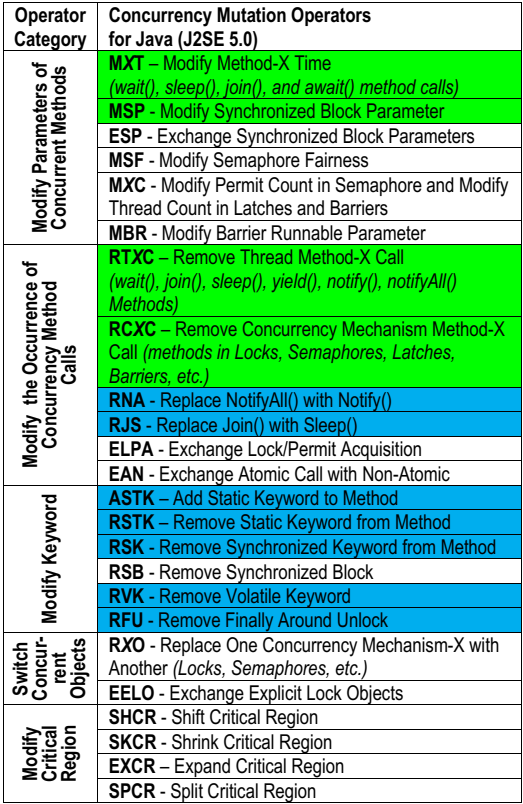
\includegraphics[scale = 0.65]{MO_categories.png}
    \caption{List of concurrency mutation operators devised by \citet{bradbury06} The green highlighted operators have been fully implemented in the mutation testing tool. The blue highlighted operators could be implemented without difficulty.}
    \label{table:MO_cat}
\end{table}

\begin{table}
    \centering
    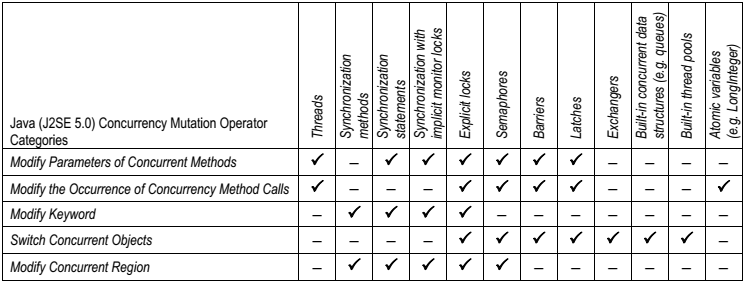
\includegraphics[scale = 0.85]{MO_features.png}
    \caption{The relationship between new mutation operators for concurrency and the concurrency features provided by J2SE 5.0 \citep{farchi03}.}
    \label{table:MO_features}
\end{table}


\end{document}
